\documentclass[11pt, oneside]{article}

%: Packages importeren
\usepackage[parfill]{parskip}    		% Activate to begin paragraphs with an empty line rather than an indent
\usepackage{graphicx,wrapfig,subcaption}
\graphicspath{{./figs/}}
\usepackage{geometry}
\geometry{bmargin=4cm}
\usepackage{amssymb}
\usepackage{amsmath}
\usepackage{hyperref}
\usepackage{multirow} 					% Tabelopmaak
\usepackage[dutch]{babel}
\usepackage{amsthm}					% Maak een counter voor lemma's en definities
\usepackage{tikz}
\usetikzlibrary{calc,patterns}
\usepackage{calc}
\usepackage{xparse} %meerdere optionele argumenten voor macros
\usepackage{pgfplots}

\usepackage{mathtools}
\DeclarePairedDelimiter\ceil{\lceil}{\rceil}
\DeclarePairedDelimiter\floor{\lfloor}{\rfloor}

\newcommand\aesuper[2][0.90]{^{\scalebox{#1}{$\scriptstyle#2$}}} % super-super-super script
\newcommand{\myparagraph}[1]{\paragraph{#1}\mbox{}\\} %start elke paragraaf op een nieuwe regel

%: Taartverdeling maken met TikZ
\NewDocumentCommand{\verdeeltaart}{O{black} O{black} O{black} O{1} m m m m m}{ % kleur S1, kleur S2, kleur S3, straal, positie, X1, X2, X3, caption tekst
    \coordinate (M) at (3*#5,0);
    \coordinate(A) at ($(M) + (0:#4)$);
    \coordinate(a) at ($(M) + (360*#6/\the\numexpr#6+#7+#8\relax/2:#4/2)$);
    \coordinate(B) at ($(M) + (360*#6/\the\numexpr#6+#7+#8\relax:#4)$);
    \coordinate(b) at ($(M) + (360*#7/\the\numexpr#6+#7+#8\relax/2+360*#6/\the\numexpr#6+#7+#8\relax :#4/2)$);
    \coordinate(C) at ($(M) + (-360*#8/\the\numexpr#6+#7+#8\relax:#4)$);
    \coordinate(c) at ($(M) + (-360*#8/\the\numexpr#6+#7+#8\relax/2:#4/2)$);
    \draw (M) circle (#4cm);
    \draw[dashed] ($(M)-(0,1.5)$) node {#9}
    %\draw[dashed] ($(M)-(0,1.5)$) node {\IfBooleanTF #8{Enzovoorts}{#9}}
        (M) -- (A)
        (a) node {{\color{#1}$S_1$}}
        (M) -- (B)
        (b) node {{\color{#2}$S_2$}}
        (M) -- (C)
        (c) node {{\color{#3}$S_3$}};
}

%: Automatische lay-out voor Python code
\usepackage{listings}
\definecolor{codestring}{RGB}{0, 170, 0}
\definecolor{codecomment}{RGB}{221, 0, 0}
\lstset{
    frame=single,
    framexleftmargin=2pt,
    language=Python,
    showstringspaces=false,
    columns=flexible,
    basicstyle={\small\ttfamily},
    numbers=left,
    numberstyle=\small,
    keywordstyle=\color{blue},
    commentstyle=\color{codecomment}, %dkgreen
    stringstyle=\color{codestring}, %mauve
    breaklines=true,
    breakatwhitespace=true,
    tabsize=3
}

\usepackage{mdframed}

%: Automatische lay-out voor protocollen
\mdfdefinestyle{protocol}{%
    linecolor=gray,
    outerlinewidth=1pt,
    roundcorner=20pt,
    innertopmargin=\baselineskip,
    innerbottommargin=\baselineskip,
    innerrightmargin=20pt,
    innerleftmargin=20pt,
    backgroundcolor=gray!30!white}
    
%: Achtergrondafbeelding voor de omslagpagina
\usepackage{eso-pic}
    \newcommand\BackgroundPic{%
    \put(0,0){%
    \parbox[b][\paperheight]{\paperwidth}{%
    \vfill
    \centering
    \includegraphics[height=\paperheight,%
    keepaspectratio]{cover3.jpg}%
    \vfill
}}}

%: Document informatie
\title{Dagelijkse toepassingen van de speltheorie}
\date{\today}
\author{Dani\"el Kuckartz}

%: Begin van het document
\begin{document}
\selectlanguage{dutch}
\pagenumbering{gobble}

\begin{titlepage}
    \AddToShipoutPicture*{\BackgroundPic}
    \newgeometry{top=2cm}
    \center
    \textsc{\LARGE Baudartius College}\\[1.2cm]
    \rule{\linewidth}{0.5mm}\\[0.4cm]
    { \huge \bfseries Dagelijkse toepassingen van de speltheorie}\\[0.4cm]
    \rule{\linewidth}{0.5mm}\\[1.2cm]
    
    \begin{minipage}{0.4\textwidth}
        \begin{flushleft} \large
            \emph{Auteur, klas:}\\
            Dani\"el Kuckartz, V6a
        \end{flushleft}
    \end{minipage}
    ~
    \begin{minipage}{0.4\textwidth}
        \begin{flushright} \large
            \emph{Begeleider:} \\
            J. Schipper
        \end{flushright}
    \end{minipage}\\[1.5cm]
    
    {\large \today}
    \vfill
    \restoregeometry
\end{titlepage}

\pagenumbering{arabic}
\section*{Voorwoord}
In dit profielwerkstuk ga ik specifiek in op verdeelproblemen, een tak van speltheorie. In eerste instantie was ik van plan om de (dagelijkse) toepassingen van de speltheorie als uitgangspunt voor het werkstuk te nemen, maar bij nader inzien bleek dit te breed te zijn voor een werkstuk als dit. Ik heb me daarom beperkt tot de verdeelproblemen. Voor een goed begrip van de verdeelproblemen is het nodig te weten wat de speltheorie inhoudt. In hoofdstuk \ref{sec:speltheorie} besteed ik daar aandacht aan. In hoofdstuk \ref{sec:cake_cutting} ga ik nader in op de Fair Cake Cutting. In hoofdstuk \ref{sec:bankroet} behandel ik bankroetproblemen, dat net als Fair Cake Cutting een type verdeelprobleem is. Ik heb daarbij veelvuldig geprogrammeerd in Python en de codes zo overzichtelijk mogelijk weergegeven en uitgelegd. Tot slot zal in hoofdstuk \ref{sec:democratie} theorie over politieke kiessystemen aan bod komen.
 
Bij het schrijven van dit profielwerkstuk heb ik grote zorg besteed aan een prettige lay-out. Verder heb ik zo veel mogelijk figuren ingevoegd ter bevordering van het begrijpen van dit abstracte onderwerp. Ik hoop dat je veel plezier zult hebben aan het lezen van mijn werkstuk en natuurlijk ook dat je er nog wat van leert!
\newpage
\tableofcontents
\newpage

%: Maak automatische counters aan voor de volgende onderdelen
\newtheorem{theorem}{Stelling}%[section]
\newtheorem{lemma}[theorem]{Lemma}
\newtheorem{proposition}[theorem]{Bewering}
\newtheorem{eis}{Eigenschap}[section]
\newtheorem{step}{Stap}

\section{Wat is speltheorie?}
\label{sec:speltheorie}
De speltheorie richt zich op het vinden van de beste strategie voor personen die in een sociaal conflict zijn geraakt. Deze personen worden in de speltheorie veelal aangeduid met het woord "spelers". Spelers kunnen bijvoorbeeld concurrerende winkelketens zijn, maar ook oorlogvoerende landen of zelfs de natuur (lees: het toeval). Speltheorie is dus erg breed en het vindt zijn toepassingen dan ook in allerlei disciplines waaronder economie, zuivere wiskunde, politiek, psychologie, marketing en biologie. Het betreffende sociale conflict wordt het spel genoemd. Hier komt de term speltheorie vandaan. Ten onrechte denken de meeste mensen dat speltheorie een (wiskundige) theorie is achter spelletjes zoals boter-kaas-en-eieren of mastermind.\footnote{De wiskunde achter spelletjes als boter-kaas-en-eieren zou ik willen plaatsen in het deelgebied recreatieve wiskunde, omdat toepassingen van deze wiskunde moeilijk te vinden zijn. Dat neemt niet weg dat recreatieve wiskunde een uitstekende manier is om te leren hoe je wiskundige problemen op kunt lossen.}

Sociale processen zijn heel moeilijk te begrijpen, laat staan om te analyseren. Er bestond dan ook geen goede methode voor totdat de speltheorie ontstond toen John van Neumann en Oskar Morgenstern als eersten het verband legden tussen wiskundige strategie\"en en het oplossen van sociale conflicten. In 1944 publiceerden zij "Theory of Games and Economic Behavior" waarin ze hun visie geven, definities formuleren en veel stellingen bewijzen die nu nog ten grondslag liggen aan de speltheorie. Vanwege de complexiteit van de meeste spellen hebben zij een aantal belangrijke aannames genomen om deze spellen analyseerbaar te maken. Zo zijn de spelers altijd razend intelligent, rationeel en hebben zij een onuitputtelijk geheugen. We gaan er dus van uit dat spelers nooit menselijke fouten maken. Ook willen alle spelers altijd hun winst maximaliseren en spelen ze optimaal om dat te bereiken.

\subsection{Deelgebieden van de speltheorie}
Verschillende soorten spellen vereisen verschillende benaderingen. De relaties tussen de spelers van een spel is een belangrijke eigenschap voor de classificatie van dat spel. In co\"operatieve spellen kunnen spelers samenwerken met andere spelers en mogen soms bindende afspraken maken. In de niet-co\"operatieve spellen speelt ieder voor zich. Een tweepersoonsspel waarbij de belangen van de spelers tegengesteld aan elkaar zijn, heet een nulsomspel. De winst van de ene speler is het verlies van de andere, ofwel: de som van de winsten van beide spelers is altijd nul. Vaak zijn recreatieve spelletjes nulsomspellen, evenals oorlogsvoering. Verder heeft een spel volmaakte informatie als alle spelers voorzien zijn van alle mogelijke informatie. Als gevolg hiervan weet ook iedere speler wat elk van zijn medespelers weet en weet hij ook dat zijn medespelers weten wat hij zelf weet. 
Spellen kunnen ook geclassificeerd worden op basis van het beoogde doel van het spel. Voorbeelden hiervan zijn het verdeelprobleem, huwelijksprobleem, optimaal stoppen en het verkiezingsprobleem.

\subsection{Verdeelproblemen}
Zoals de term al doet vermoeden, gaat het er bij dit soort problemen om een winst te verdelen onder de spelers zodanig dat iedereen tevreden is. Er zijn veel verschillende soorten verdeelproblemen en elk daarvan heeft meerdere oplossingen. Een oplossing is geen specifieke verdeling, maar een strategie die beschrijft wat elke speler moet doen om gezamenlijk tot een eerlijke verdeling te kunnen komen. Een protocol is hetzelfde als een strategie, behalve dat de spelers van een protocol af mogen wijken. Echter als het protocol goed in elkaar zit, d.w.z. het is een oplossing van het betreffende verdeelprobleem, dan zal geen speler er baat bij hebben om af te wijken van het protocol.

%: Fair Cake Cutting
\clearpage
\section{Fair Cake Cutting}
\label{sec:cake_cutting}
Ik zal eerst verdeelproblemen behandelen waarbij er een taart eerlijk verdeeld moet worden. De bekende Engelstalige term voor deze problemen is "Fair Cake Cutting". De taart is een algemeen erkend metafoor binnen de speltheorie die de eigenschappen van dit verdeelprobleem eenvoudig illustreert. Het verdelen van eigendommen van een scheidend echtpaar of het verdelen van Berlijn onder de Fransen, Engelsen, Amerikanen en Russen gaat op dezelfde manier. Bij het snijden van de taart gaat niets verloren en elke speler kan snijden zonder snijfouten te maken \textit{(rationaliteit)}. De totale waarde van de taart is $T$. Er zijn $n$ spelers en we noemen ze achtereenvolgend $S_1, S_2, \ldots, S_n$. $S_i$ is een willekeurige speler in het hiervoorgenoemde rijtje, in formulevorm: $S_i$ met $1 \leq i \leq n$. In het vervolg zal ik voor het gemak de voorwaarde $1 \leq i \leq n$ bij $S_i$ weglaten. De waarde van het stuk taart dat $S_i$ denkt te hebben gekregen, noemen we $X_i$. De waarde die $S_i$ aan een stuk taart, zeg $A$, geeft, noemen we $v_i(A)$. In tegenstelling tot het verdelen van een geldbedrag weten we bij onze taart niet of alle stukken taart in werkelijkheid precies $\frac{1}{n}$ waard zijn. Het gaat er dus om wat iedere speler denkt te hebben gekregen en niet om wat ze in werkelijkheid hebben gekregen. Daarom kan het voorkomen dat $\sum_{i=1}^{n} v_i(X_i) > T$.

\begin{figure}[htb]
    \begin{center}
        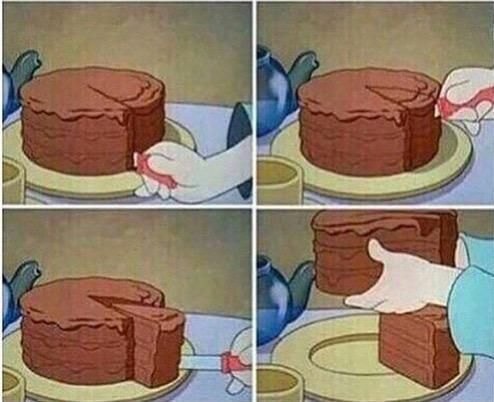
\includegraphics[width=200pt]{cake-cutting-joke.jpg}
        \caption{Hoe elke rationele speler een taart zou \underline{willen} verdelen.}
    \end{center}
\end{figure}

%: De snijd-en-kies methode
\subsection{De snijd-en-kies methode}
Het beroemde snijd-en-kies protocol werkt relatief goed in verhouding tot zijn eenvoud. Het is uitstekend te gebruiken bij twee gelijkwaardige spelers die niet al te veel eisen stellen. De enige eis die beide spelers stellen, is dat ze minimaal de helft van de taart willen. In andere woorden: de verdeling moet proportioneel zijn. 

\begin{eis}{Een verdeling is \textbf{proportioneel} als geldt dat $v_i(X_i) \geq \frac{1}{n}$} \end{eis}

Het snijd-en-kies protocol gaat als volgt.\\
\begin{mdframed}[style=protocol]
    \begin{step}{$S_1$ maakt een verdeling waarvan hij denkt dat beide delen $\frac{1}{2}$ waard zijn.} \end{step}
    \begin{step}{$S_2$ kiest een stuk. Als hij denkt dat de stukken ongelijk verdeeld zijn, dan kiest hij het grootste en is tevreden.} \end{step}
    \begin{step}{$S_1$ neemt het andere stuk. Hij heeft gesneden, dus is tevreden over elk stuk.} \end{step}
\end{mdframed}

\noindent
Het nadeel van het vorige protocol is dat het niet uitbreidbaar is naar drie personen. 

%: Het Steinhaus protocol
\subsection{Het Steinhaus protocol} 
Het Steinhaus protocol werkt ongeveer op dezelfde manier als de snijd-en-kies methode, maar dan met precies drie personen.\\

\begin{mdframed}[style=protocol]
    \setcounter{step}{0}
    \begin{step}{$S_1$ maakt een verdeling waarvan hij denkt dat alle delen $\frac{1}{3}$ waard zijn. Hij wil dus alle stukken wel hebben} \end{step}
    \begin{step}
                {Als $S_2$ minstens twee van de stukken wel wil, dan kiezen $S_3$, $S_2$ en $S_1$ in die volgorde een stuk.\\    
                Als $S_2$ maar \'e\'en stuk wil en $S_3$ minstens twee van de stukken wel wil, dan kiezen $S_2$, $S_3$ en $S_1$ in die volgorde een stuk.\\
                Als $S_2$ en $S_3$ beiden \'e\'en stuk willen hebben, maar verschillende, dan kiezen ze hun stuk en krijgt $S_1$ het overige stuk. \\
                Als $S_2$ en $S_3$ allebei maar \'e\'en en hetzelfde stuk willen, dan kiest $S_1$ een stuk dat ze beide niet willen en verdelen $S_2$ en $S_3$ de overige twee stukken volgens de snijd-en-kies methode voor twee spelers.}
    \end{step}
\end{mdframed}

Dit protocol werkt, omdat de spelers in een zodanige volgorde kiezen dat er telkens minimaal \'e\'en stuk overblijft die de speler die aan de beurt is wel wil hebben. Bij deze methode hoeft er maar heel weinig gesneden te worden om tot een verdeling te komen. De verdeling hoeft helaas toch niet altijd helemaal eerlijk te zijn, want het Steinhaus protocol is niet jaloezie-vrij: er zou iemand kunnen zijn die denkt dat zijn stuk kleiner is dan dat van de ander en dat oneerlijk vindt. In figuur 2 wordt dit ge\"illustreerd. Het snijd-en-kies protocol vergt nog minder sneden en is wel jaloezie-vrij.

\begin{eis}{Een verdeling is {\bf jaloezie-vrij} als $v_i(X_i) \geq v_i(X_j)$ voor $1 \leq i \leq n$ en $1 \leq j \leq n$. Met andere woorden: een verdeling is jaloezie-vrij als iedereen denkt dat zijn eigen stuk minimaal net zo groot is als de stukken van de medespelers.} \end{eis}

\begin{figure}[htbp]
\centering
 \resizebox {\linewidth}{!}{
        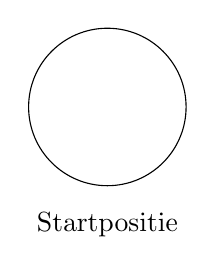
\begin{tikzpicture}
            \draw (0,0) circle (1cm) 
                (0,-1.5) node {Startpositie};
            \verdeeltaart{1}{1}{1}{1}{Situatie 1}
            \verdeeltaart[green][white][white]{2}{1}{1}{1}{Situatie 2}
            \verdeeltaart[red][green][green]{3}{3}{2}{4}{Situatie 3}
            \verdeeltaart[green][green][red]{4}{2}{3}{4}{Enzovoorts}
        \end{tikzpicture}
        }
\caption{Illustratie van het Steinhaus-protocol}
\label{fig:taart1}
\end{figure}

In situatie 1 van figuur~\ref{fig:taart1} snijdt $S_1$ de taart volgens hem in drie gelijke stukken. Echter de beide andere spelers denken daar anders over en willen allebei absoluut het stuk aan de linkerkant. In situatie 2 neemt $S_1$ een van de stukken die beide andere spelers niet willen hebben. Vervolgens snijdt $S_2$ de resterende twee stukken zodat hij denkt dat de stukken gelijk zijn. Echter $S_1$ denkt dat $S_2$ niet eerlijk heeft verdeeld en dat een van de twee stukken groter is dan het stuk dat $S_1$ zelf heeft. Opnieuw bijsnijden volgens de snijd-en-kies methode heeft geen zin, aangezien er dan altijd een speler buiten beschouwing wordt gelaten, waardoor die speler altijd oneens kan zijn met de nieuwe verdeling. Herhalen van het Steinhaus protocol heeft evenmin zin, want die methode is niet jaloezie-vrij.

%: Het Selfridge-Conway protocol
\subsection{Het Selfridge-Conway protocol}
Het Selfridge-Conway protocol werkt enkel voor $n = 3$ en bestaat uit twee gedeelten. Beide delen van het protocol zijn jaloezie-vrij, waardoor het geheel ook jaloezie-vrij is.\\

\begin{mdframed}[style=protocol]
    \setcounter{step}{0}
     \myparagraph{Deel 1}
    \begin{step}{$S_1$ maakt een verdeling waarvan hij denkt dat alle delen $\frac{1}{3}$ waard zijn.} \end{step}
    \begin{step}{Noem het stuk taart dat $S_2$ het grootst vindt even $A$, het een-na-grootste stuk $B$ en het kleinste stuk $C$. $S_2$ snijdt een stuk $M$ af van $A$, zodat $v_2(A) = v_2(B)$ Laat $M$ even buiten beschouwing tot deel 2 van het protocol.} \end{step}
    \begin{step}{$S_3$, $S_2$ en $S_1$ kiezen in die volgorde een stuk onder voorwaarde dat  $S_2$ het stuk $A$ neemt als $S_3$ die niet heeft gekozen.} \end{step}
    \myparagraph{Deel 2}
    \begin{step}{Noem de speler die $A$ heeft gekregen even $S_A$ en de speler die het {\bf niet} heeft gekregen en niet $S_1$ is even $S_{\lnot A}$. $S_{\lnot A}$ maakt een verdeling van $M$ waarbij hij denkt dat alle delen $\frac{1}{3}$ waard zijn.} \end{step}
    \begin{step}{Eerst kiest $S_A$ een stuk van $M$, vervolgens $S_1$ en tot slot neemt $S_{\lnot A}$ het laatste stuk.} \end{step}
\end{mdframed}

\myparagraph{Bewijs dat deel 1 van dit protocol jaloezie-vrij is}
\begin{itemize}
    \item \ldots voor $S_3$: het is jaloezie-vrij voor $S_3$, omdat hij als eerste mag kiezen. Hij kiest dan het stuk dat hij het grootst vindt.
    \item \ldots voor $S_1$: $S_1$ heeft in stap 1 alle stukken even groot gesneden, dus hij wil alle stukken wel hebben, behalve het stuk $A$. Echter door de voorwaarde in stap 3 kan het niet gebeuren dat $S_1$ dit stuk krijgt.
    \item \ldots voor $S_2$:
    	\begin{itemize}
		\item Stel dat $S_3$ het stuk $C$ kiest, dan is er geen probleem voor $S_2$, want dan moet hij $A$ kiezen en $v_2(A) = v_2(B) \leq v_2(C)$
      		\item Stel dat $S_3$ het stuk $B$ kiest, dan is dat ook geen probleem, want dan moet $S_2$ $A$ kiezen en $v_2(A) = v_2(B) \leq v_2(C)$
      		\item Stel dat $S_3$ het stuk $A$ kiest, dan kiest $S_2$ het stuk $B$. Hij is hiermee tevreden, want $v_2(B) = v_2(A) \leq v_2(C)$
        	\end{itemize}   
\end{itemize}

Het lijkt alsof we na stap 3 weer terug bij af zijn: een stuk, kleiner weliswaar, verdelen over drie spelers. Echter dat is niet waar, want nu kan $S_1$ niet jaloers worden op $S_A$. Immers in deel 1 van het protocol geldt $v_1(A) + v_1(M) = v_1(X_1)$
\begin{lemma}$S_1$ is niet jaloers op $S_A$\end{lemma}

\myparagraph{Bewijs dat deel 2 van dit protocol jaloezie-vrij is}
\begin{itemize}
    \item \ldots voor $S_A$: hij mag als eerste kiezen, dus hij is tevreden.
    \item \ldots voor $S_1$: hij mag v\'o\'or $S_{\lnot A}$ kiezen en is niet jaloers op $S_A$ (Lemma 1), dus hij is tevreden.
    \item \ldots voor $S_{\lnot A}$: hij heeft $M$ gesneden, dus hij is tevreden met elk stuk.
\end{itemize}

Over het algemeen kun je twee jaloezie-vrije oplossingen, d.w.z. protocollen, als het ware bij elkaar optellen en daaruit een jaloezie-vrije oplossing krijgen. Dit wordt additiviteit genoemd. Als een functie of bewerking additief is, geldt: $f(a) + f(b) = f(a+b)$. Omdat zowel deel 1 als deel 2 van het Selfridge-Conway protocol jaloezie-vrij zijn, is het protocol in zijn geheel ook jaloezie-vrij.

\begin{figure}[htb]
\centering
 \resizebox {\linewidth}{!}{
        \begin{tikzpicture}
            \verdeeltaart[green][green][green]{1}{1}{1}{1}{}
            \verdeeltaart[green][green][green]{3}{1}{1}{1}{}
            \verdeeltaart[green][green][green][1.414]{5}{1}{1}{1}{}
            \node at (6,0) {+};
            \node at (12,0) {=};
        \end{tikzpicture}
        }
\caption{Illustratie van het begrip additiviteit}
\label{fig:additief}
\end{figure}

\color{black}

%: Het aantal keer snijden
\subsection{Complexiteit}
Het is wenselijk dat we bij een protocol zo min mogelijk hoeven te snijden. Immers snijden kost tijd en tijd is soms kostbaar, zoals blijkt in figuur \ref{fig:bijna_koud}.

\begin{figure}[htb]
    \begin{center}
        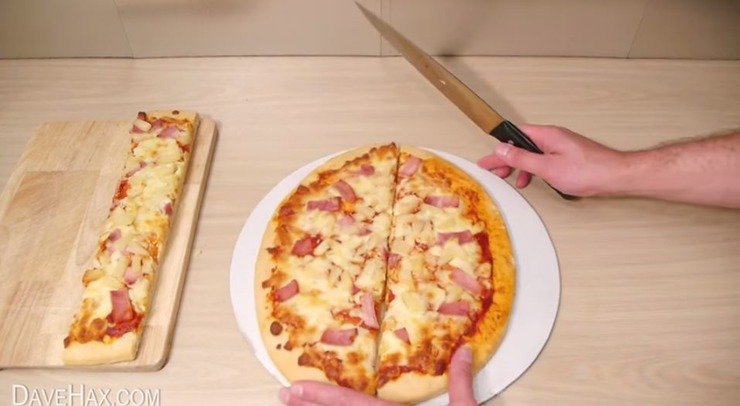
\includegraphics[width=200pt]{rond_recht.jpg}
        \caption{De pizza is al bijna koud \ldots}
        \label{fig:bijna_koud}
    \end{center}
\end{figure}

Het verdelen van een ronde taart op de huiselijke manier zoals schematisch getekend is in figuur \ref{fig:taartvormen}a moet altijd precies \'e\'en keer vaker gesneden worden dan een vergelijkbare verdeling van een rechthoekige taart (figuur \ref{fig:taartvormen}b) of een taart van een wiskundige (figuur \ref{fig:taartvormen}c). Dit komt omdat het beginpunt in de twee laatstgenoemde taarten al is aangegeven door de rand van de taart. Het blijkt in verband met formules gemakkelijker te zijn om het maximaal benodigd aantal keer snijden te tellen in het geval van taart \ref{fig:taartvormen}b of taart \ref{fig:taartvormen}c. Verder is het vooral voor de niet-wiskundige lastig gebleken om taart \ref{fig:taartvormen}c eerlijk te verdelen zonder hulp van een rekenmachine met goniometrische functies. Daarom ga ik in het vervolg bij het aantal keren snijden uit van een rechthoekige taart zoals in figuur \ref{fig:taartvormen}b.

\begin{figure}[htb]
\centering
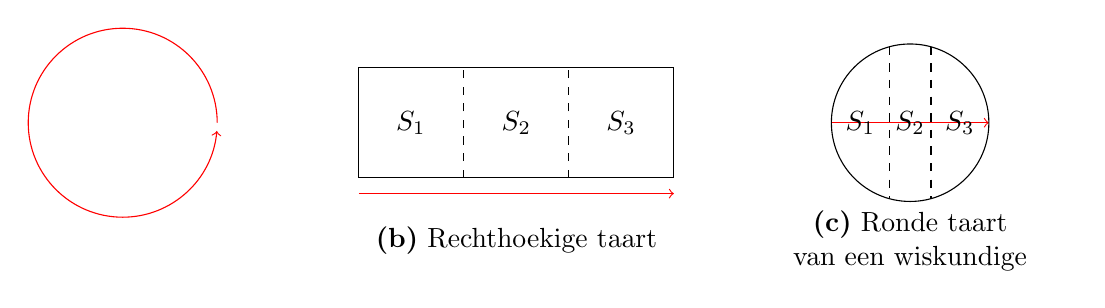
\begin{tikzpicture}
    \verdeeltaart{0}{1}{1}{1}{\textbf{(a)} Ronde taart}
    \draw [->,red] (1.2,0) arc (0:355:1.2);
    
    \draw (3,-.7) rectangle (7,.7) node at (5,-1.5) {\textbf{(b)} Rechthoekige taart};
    \draw [->,red] (3,-.9) -- (7,-.9);
    \draw [dashed] (4.33,-.7) -- (4.33,.7);
    \node at (3.66,0) {$S_1$};
    \draw [dashed] (5.66,-.7) -- (5.66,.7);
    \node at (5,0) {$S_2$};
    \node at (6.33,0) {$S_3$};
    
    \draw [->,red] (9,0) -- (11,0);
    \draw [align=center, text width=4cm] (10,0) circle (1cm) node at (10,-1.5) {\textbf{(c)} Ronde taart van een wiskundige};
    \node at (9.3676,0) {$S_1$};
    \draw [dashed] (10-.2649,0.9643) -- (10-.2649,-0.9643);
    \node at (10,0) {$S_2$};
    \draw [dashed] (10.2649,0.9643) -- (10.2649,-0.9643);
    \node at (10.6325,0) {$S_3$};
\end{tikzpicture}
\caption{De ronde taart moet drie keer gesneden worden en de vergelijkbare rechthoekige taart precies een keer minder.}
\label{fig:taartvormen}
\end{figure}

In de informatica en wiskunde wordt gebruik gemaakt van de grote-O-notatie. Deze notatie geeft de (tijds)complexiteitsgraad van algoritmen aan als een parameter, indien aanwezig, naar oneindig toe gaat. Anders gezegd: met de grote-O-notatie kunnen we bij benadering de groei van het aantal keren snijden weergeven bij een groot aantal spelers. Kortweg noemen we dit de complexiteit van het protocol. Een hoge complexiteit betekent dat er veel gesneden moet worden. Het voordeel van deze notatie is dat de waarde ervan in de meeste gevallen een basisfunctie is, zoals $n^2$ of $\log{n}$, waardoor we een goed beeld krijgen van de groeisterkte. In sectie \ref{sec:banach_knaster} wordt deze notatie gebruikt en de waarde ervan beredeneerd, dus ik hoop dat het begrip dan duidelijker wordt.

\begin{eis}
We willen dat een protocol een lage complexiteit heeft, oftewel dat het zo min mogelijk aantal keer snijden vergt. Deze waarde wordt berekend in het ergste geval, d.w.z. elke speler snijdt een stuk taart bij zodra hij er de kans voor krijgt. De waarde wordt weergegeven in de grote-O-notatie.
\end{eis}

%: Het Banach-Knaster Laatste Bijsnijder protocol
\subsection{Het Banach-Knaster Laatste Bijsnijder protocol}
\label{sec:banach_knaster}
Met het Banach-Knaster protocol dat door de wiskundigen Stefan Banach en Bronislaw Knaster bedacht werd, kan men proportioneel verdelen onder $n$ spelers. \\\begin{mdframed}[style=protocol]
    \setcounter{step}{0}
    \begin{step}{$S_1$ snijdt een stuk $A$ zo dat $v_1(A) = \frac{1}{n}$} \end{step}
    \begin{step}{De spelers $S_2$ tot en met $S_n$ krijgen om de beurt de keuze om bij te snijden (als hij denkt dat het stuk minstens $\frac{1}{n}$ waard is) of te passen (als hij denkt dat het minder dan $\frac{1}{n}$ waard is. De afgesneden stukjes worden bij de rest van de taart gevoegd.} \end{step}
    \begin{step}{De speler die als laatste (bij)gesneden heeft, krijgt het stuk en verlaat het spel.} \end{step}
    \begin{step}{Herhaal stap 1 tot en met stap 3 totdat er nog maar 1 speler over is. Hij krijgt de rest van de taart.} \end{step}
\end{mdframed}

Het geheim achter de werking van het protocol ligt in de recursiviteit\footnote{Een algoritme waarbij een antwoord gevonden wordt met behulp van een eerder gevonden antwoord heet een recursief algoritme. In bijlage \ref{sec:AppRecursief} staat het begrip recursie uitgelegd aan de hand van een voorbeeld.} in stap 3. Iedere ronde verlaat er namelijk een tevreden speler het spel en wel zo dat alle andere spelers ook tevreden blijven. Een speler zal bijsnijden als hij denkt dat het stuk groter is dan $\frac{1}{n}$ en passen als hij denkt dat het kleiner is. Het protocol is proportioneel en jaloezie-vrij. Kortom, dit is een zeer krachtig protocol. Het jammere is dat er erg veel gesneden moet worden: maximaal $\frac{n(n+1)}{2}$ keer. Wordt $n$ heel groot, dan mogen we $n+1$ verwaarlozen tot $n$. De orde van grootte verandert ook niet als we de noemer weglaten. Dus $\lim_{n \to \infty} f(n) = n^2$ met $f(n)$ het maximaal aantal keer snijden bij n spelers. In big-O-notatie wordt dat dan $O(n^2)$. Dit is een snelle groei. Ik moet erbij vermelden dat de taart nog steeds metaforisch is en het snijden dus ook. Bij een echte taart kun je niet zo gemakkelijk stukken weer samenvoegen, omdat je geen vaste hand hebt en de taart bij zeer dunne plakjes instabiel wordt. Het is dan aan te raden slechts aanduidingen te tekenen of kerven op de plaatsen waar je zou willen snijden. Snijden doe je dan pas als de uiteindelijke verdeling gemaakt is. In dat geval geldt altijd dat er $O(n)$ keer gesneden moet worden. Deze complexiteitsgraad noemen we in de context van Fair Cake-Cutting minimaal, want er moet altijd $n$ keer gesneden worden wil iedereen een stuk kunnen oppakken.

\clearpage %% lelijke oplossing
\subsection{Het Dubins-Spanier protocol}

\myparagraph{Het continue protocol}
\begin{mdframed}[style=protocol]
    \setcounter{step}{0}
    \begin{step}{Een onpartijdige buitenstaander verschuift een mes van links naar rechts over een rechthoekige taart zoals afgebeeld in figuur \ref{fig:taartvormen}.} \end{step}
    \begin{step}{Terwijl de buitenstaander dit doet, hebben alle spelers het recht om "STOP" te roepen. Als dat gebeurt, krijgt de speler die riep het stuk taart links van het mes en hij verlaat het spel.} \end{step}
\end{mdframed}

Er wordt hier in totaal $n$ keer gesneden. Merk op dat dit geen protocol is zoals we eerder gezien hebben, want deze methode maakt gebruik van een continu tijdselement. Je zou dus ook kunnen zeggen dat het oneindig lang duurt om het mes van de buitenstaander te verschuiven, dus $O(\infty)$. Het heeft ook het vervelende bijgevolg dat alle spelers bij een dergelijke verdelingsprocedure bij elkaar moeten zijn. Leuk voor in de kroeg, behalve als daar wiskundigen aanwezig zijn (wiskundigen gaan soms ook naar de kroeg). Gelukkig kost het niet veel moeite om deze methode discreet te maken.

\myparagraph{Het discrete protocol}
\begin{mdframed}[style=protocol]
    \setcounter{step}{0}
    \begin{step}{Elke speler tekent een streep op de plek waar zijn $\frac{1}{n}$ grenspunt ligt.} \end{step}
    \begin{step}{Snijd de taart langs de meest linkse streep en geef dat stuk aan de bijbehorende speler} \end{step}
    \begin{step}{Herhaal stap 1 en stap 2 totdat er nog maar 1 speler over is. Hij krijgt de rest van de taart.} \end{step}
\end{mdframed}

Het nadeel van het discrete protocol is er veel gesneden moet worden, althans als je streepjes zetten ook telt als snijden. Omdat de taart metaforisch wordt gebruikt, tel ik streepjes zetten mee als snijden. Er moet dan $O(n^2)$ keer gesneden worden, niet meer en niet minder.

Verder is dit protocol wel proportioneel, maar niet jaloezie-vrij. Zodra de eerste speler namelijk uit het spel is, geldt $v_1(X_1) = \frac{1}{n}$. Stel dat hij nog een keer een streepje zou zetten en dat hij weer het meest linkse streepje heeft gezet. Omdat hij uit het spel is, wordt zijn streepje genegeerd en gaat het het stuk taart waarvan hij denkt dat het weer $\frac{1}{n}$ waard is, inclusief het interval tussen zijn streepje en het tweede streepje van links, naar een andere speler. Er geldt nu $v_1(X_2) = \frac{1}{n} + dT > \frac{1}{n} = v_1(X_1)$. Dus $v_1(X_1) < v_1(X_2)$, met andere woorden: $S_1$ is jaloers op $S_2$.

\subsection{Het Even-Paz deel-en-bemachtig protocol}
De wiskundigen Even en Paz zochten gericht naar een protocol dat zo min mogelijk keer snijden zou vergen. Ze hebben het volgende protocol ontwikkeld dat optimaal is voor $n > 4$. Voor dit protocol zijn $O(n \ln{n})$ sneden benodigd.

\paragraph{Afspraak}
$\floor*{\frac{x}{2}}$ is het hoogste natuurlijke getal kleiner dan $\frac{x}{2}$.
$\ceil*{\frac{x}{2}}$ is het kleinste natuurlijke getal groter dan $\frac{x}{2}$.\\

\begin{mdframed}[style=protocol]
    \setcounter{step}{0}
    \begin{step}{Elke speler snijdt de taart in twee\"en op de plek waar zijn $\floor*{\frac{x}{2}} / \ceil*{\frac{x}{2}}$ grenspunt ligt.} \end{step}
    \begin{step}{Geef de $\floor*{\frac{x}{2}}$ meest linkse stukjes aan de betreffende $\floor*{\frac{x}{2}}$ spelers (noem hen groep 1) en de rest van de stukjes aan de andere spelers. (noem hen groep 2)} \end{step}
    \begin{step}{Herhaal stap 1 en stap 2 in beide gevormde groepen totdat er elke groep uit slechts 1 speler bestaat.} \end{step}
    \begin{step}{Elke speler krijgt alle stukjes taart in zijn groep.} \end{step}
\end{mdframed}

\myparagraph{Bewijs dat er $O(n \ln{n})$ sneden benodigd zijn.}
De complexiteitsgraad kan begrepen worden met behulp van een binaire spelboom zoals afgebeeld in figuur \ref{fig:Even-Paz-spelboom}. Iedere keer dat er een groep in twee\"en wordt gesplitst bij stap 2 van het protocol vertakt de spelboom zich. Elk punt van de spelboom\footnote{dit zijn de plaatsen waar vertakkingen plaatsvinden. In figuur \ref{fig:Even-Paz-spelboom} zijn alle punten aangegeven met een zwarte cirkel.} representeert een bepaalde groep op een bepaald moment. In elk punt snijdt elke speler van de betreffende groep precies \'e\'en keer. Omdat er geen spelers verloren gaan, is het aantal keer dat gesneden wordt in elke laag van de spelboom\footnote{Een laag van een spelboom is een horizontale rij van punten van een spelboom, ze hebben dezelfde diepte. In figuur \ref{fig:Even-Paz-spelboom} is dat bijvoorbeeld de rij met alle $\frac{n}{2^2}$-punten.} gelijk aan $n$. Na $\ln{n}$ lagen van de spelboom bestaan alle groepen uit 1 speler. De diepte van de spelboom\footnote{De diepte van een binaire spelboom is het aantal lagen van die spelboom.} is daarom $\ln{n}$. Het totaal aantal keer dat gesneden wordt is de diepte van de spelboom vermenigvuldigd met het aantal keer dat gesneden wordt in elke laag van de spelboom. Dus $O(n) \cdot O(\ln{n}) = O(n\ln{n})$.

%: complexiteit binair boomdiagram
\begin {figure}[htb]
        \centering
        \resizebox {\linewidth} {!} {
            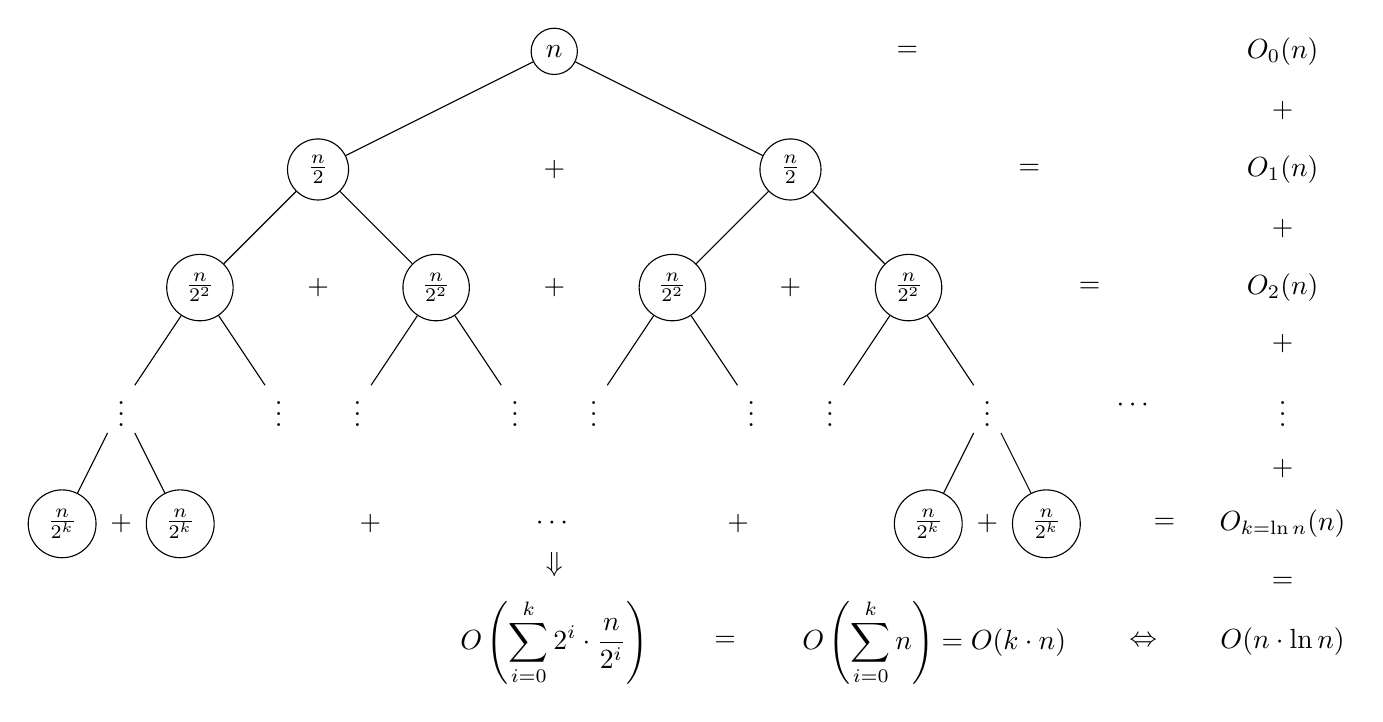
\begin{tikzpicture}[level/.style={sibling distance=60mm/#1}]
                \node [circle,draw] (z){$n$}
                  child {node [circle,draw] (a) {$\frac{n}{2}$}
                    child {node [circle,draw] (b) {$\frac{n}{2^2}$}
                      child {node {$\vdots$}
                        child {node [circle,draw] (d) {$\frac{n}{2^k}$}}
                        child {node [circle,draw] (e) {$\frac{n}{2^k}$}}
                      } 
                      child {node {$\vdots$}}
                    }
                    child {node [circle,draw] (g) {$\frac{n}{2^2}$}
                      child {node {$\vdots$}}
                      child {node {$\vdots$}}
                    }
                  }
                  child {node [circle,draw] (j) {$\frac{n}{2}$}
                    child {node [circle,draw] (k) {$\frac{n}{2^2}$}
                      child {node {$\vdots$}}
                      child {node {$\vdots$}}
                    }
                  child {node [circle,draw] (l) {$\frac{n}{2^2}$}
                    child {node {$\vdots$}}
                    child {node (c){$\vdots$}
                      child {node [circle,draw] (o) {$\frac{n}{2^k}$}}
                      child {node [circle,draw] (p) {$\frac{n}{2^k}$}
                        child [grow=right] {node (q) {$=$} edge from parent[draw=none]
                          child [grow=right] {node (q) {$O_{k = \ln n}(n)$} edge from parent[draw=none]
                            child [grow=up] {node (r) {$\vdots$} edge from parent[draw=none]
                              child [grow=up] {node (s) {$O_2(n)$} edge from parent[draw=none]
                                child [grow=up] {node (t) {$O_1(n)$} edge from parent[draw=none]
                                  child [grow=up] {node (u) {$O_0(n)$} edge from parent[draw=none]}
                                }
                              }
                            }
                            child [grow=down] {node (v) {$O(n \cdot \ln n)$}edge from parent[draw=none]}
                          }
                        }
                      }
                    }
                  }
                };
                \path (a) -- (j) node [midway] {+};
                \path (b) -- (g) node [midway] {+};
                \path (k) -- (l) node [midway] {+};
                \path (k) -- (g) node [midway] {+};
                \path (d) -- (e) node [midway] {+};
                \path (o) -- (p) node [midway] {+};
                \path (o) -- (e) node (x) [midway] {$\cdots$}
                  child [grow=down] {
                    node (y) {$O\left(\displaystyle\sum_{i = 0}^k 2^i \cdot \frac{n}{2^i}\right)$}
                    edge from parent[draw=none]
                  };
                \path (q) -- (r) node [midway] {+};
                \path (s) -- (r) node [midway] {+};
                \path (s) -- (t) node [midway] {+};
                \path (s) -- (l) node [midway] {=};
                \path (t) -- (u) node [midway] {+};
                \path (z) -- (u) node [midway] {=};
                \path (j) -- (t) node [midway] {=};
                \path (y) -- (x) node [midway] {$\Downarrow$};
                \path (v) -- (y)
                  node (w) [midway] {$O\left(\displaystyle\sum_{i = 0}^k n\right) = O(k \cdot n)$};
                \path (q) -- (v) node [midway] {=};
                \path (e) -- (x) node [midway] {+};
                \path (o) -- (x) node [midway] {+};
                \path (y) -- (w) node [midway] {$=$};
                \path (v) -- (w) node [midway] {$\Leftrightarrow$};
                \path (r) -- (c) node [midway] {$\cdots$};
            \end{tikzpicture}
            }
        \caption{Illustratie van de complexiteitsgraad van het Even-Paz protocol met behulp van een binaire spelboom}
        \label{fig:Even-Paz-spelboom}
\end{figure}

Merk op dat het aantal spelers altijd een natuurlijk getal is. Dat heeft als gevolg dat we bijvoorbeeld in het geval van $n = 5$ niet meer helemaal te maken hebben met een binaire spelboom. Immers $5 = 2 + 3 = (1+1) + (1+2) = 1+1+1+(1+1))$, dus de spelboom is niet op elk punt even diep. Dit is ge\"illustreerd in figuur \ref{fig:spelboom_n_5}. Deze kleine fout heeft geen effect in de complexiteit, vanwege $\lim_{n \to \infty}$

\begin {figure}[htb]
        \centering
        \resizebox {100pt} {!} {
            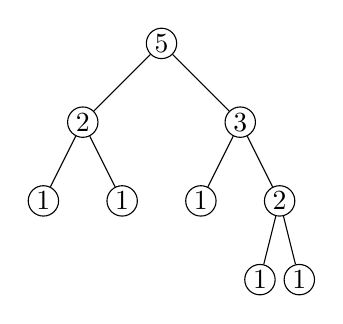
\begin{tikzpicture}[level distance=10mm]
            \tikzstyle{every node}=[circle,draw,inner sep=1pt]
            \tikzstyle{level 1}=[sibling distance=20mm]
            \tikzstyle{level 2}=[sibling distance=10mm]
            \tikzstyle{level 3}=[sibling distance=5mm]
            \node {5}
                child {node {2}
                    child {node {1}}
                    child {node {1}}
                }
                child {node {3}
                    child {node {1}}
                    child {node {2}
                        child {node {1}}
                        child {node {1}}
                    }
                };
            \end{tikzpicture}
            }
        \caption{In het geval van $n=5$ is de spelboom niet overal even diep}
        \label{fig:spelboom_n_5}
\end{figure}

%: Meer en afsluiting van fair-cake-cutting
\subsection{Grimmige taarten en kieskeurige spelers}
Ik heb nu drie wenselijke eigenschappen voor een protocol laten zien. Het protocol is \ldots
\begin{enumerate}
    \item{proportioneel}
    \item{jaloezie-vrij}
    \item{lage complexiteit}
\end{enumerate}

Als een protocol jaloezie-vrij is, dan is het ook proportioneel. Stel namelijk dat er een niet-proportioneel, jaloezie-vrij protocol bestaat, dan kunnen we wegens het niet-proportioneel-zijn aannemen dat $v_1(X_1) < \frac{1}{n}$ en wegens het  jaloezie-vrij-zijn aannemen dat $v_1(X_i) \leq v_1(X_1)$. Maar dat zou betekenen dat $\sum_{i = 1}^{n} v_1(X_i) < v_1(T) = T$. Dus niet alle stukjes taart zijn verdeeld. Dit is een tegenspraak, dus het kan niet zo zijn dat er een niet-proportioneel, jaloezie-vrij protocol bestaat.

\begin{figure}[htb]
    \begin{center}
        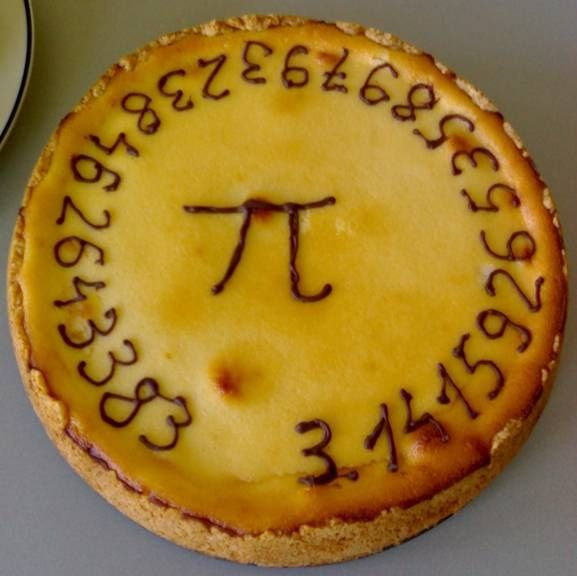
\includegraphics[width=150pt]{pi_pie.jpg}
        \caption{Dat is wel een heel bijzondere taart!}
        \label{fig:berlijn}
    \end{center}
\end{figure}

Voor $n = 2$ is er een duidelijk optimale oplossing die voldoet aan alle drie genoemde wenselijke eigenschappen. Voor $n=3$ is het Selfridge-Conway protocol de beste methode, omdat het jaloezie-vrij is en het maximaal slechts 5 keer snijden vergt. Voor grotere waarden van $n$ is moeilijk te zeggen wat een goede oplossing is, want de complexiteit is veel groter dan de minimale waarde $O(n)$. Het protocol dat het dichtst bij deze waarde komt, namelijk het Even-Paz protocol, is helaas niet jaloezie-vrij. 
%% Brams-Taylor protocol

Er zijn nog veel meer interessante taarten. Veel van deze taarten hebben eigenschappen waar de wiskundigen van vandaag nog geen grip op hebben. Enkele voorbeelden van deze eigenschappen zijn:
\begin{itemize}
    \item een protocol voor jaloezie-vrije verdelingen voor elke waarde van $n$. In 1988 werd dit probleem gemarkeerd als een van de belangrijkste wiskundige problemen van de twintigste eeuw. Pas in 1995 publiceerden S. Brams en A. D. Taylor een protocol dat hieraan voldoet. Het is gebaseerd op het protocol van Selfridge en Conway. Ze hebben patent op het protocol gekregen. De procedure kan helaas wel oneindig lang duren. Haris Aziz en Simon Mackenzie hebben in 2016 een jaloezie-vrij protocol voor elke waarde waarde van $n$ laten zien waarvan de complexiteit een bovengrens heeft\footnote{van https://arxiv.org/abs/1604.03655}\footnote{Dit is de Knuth's pijl omhoog notatie. Zijn verschijning is zeer zeldzaam \ldots}, namelijk $n\aesuper[1]{n\aesuper{n\aesuper{n\aesuper{n\aesuper{n}}}}} = n\uparrow\uparrow 6$. Of er een dergelijk protocol met een kleinere complexiteit bestaat, is nog onbekend, maar zeer gewild.
    \item de taart is samengesteld uit bijvoorbeeld vanille en chocolade. De spelers hebben elk een eigen, relatieve waardetoekenning aan de smaken, bijvoorbeeld $v_1(T_{chocolade}) = 2 \cdot v_1(T_{vanille})$. In de re\"ele wereld viel Berlijn bijvoorbeeld zeer in de smaak bij alle spelers. Zie figuur \ref{fig:berlijn}.
    \item de totale hoeveelheid taart die een bepaalde speler krijgt, hoeft niet uit een aaneengesloten stuk te bestaan. Zie nogmaals figuur \ref{fig:berlijn}.
    \item de taart is niet oneindig deelbaar. Dit is bijvoorbeeld het geval als drie studenten de kamers van een studentenhuis onder elkaar willen verdelen.
    \item een verdeelprobleem waarbij bijna-jaloezie-vrij goed genoeg is. Er bestaan namelijk combinaties van wenselijke eigenschappen die onmogelijk blijken te zijn.
    \item de spelers willen elk zo min mogelijk taart. Dit is bijvoorbeeld het geval bij het verdelen van kantoorwerk of, helemaal abstract, risico's. Omdat iedereen risico's anders inschat, is dit tevens een mooi voorbeeld voor het psychologische kenmerk van Fair Cake Cutting dat het gaat om de waarde die een persoon denkt dat een stuk waard is en niet zozeer om de werkelijke waarde van dat stuk.
    \item een protocol dat gebruik maakt van het mechanisme van bieden.
\end{itemize}

\begin{figure}[htb]
    \begin{center}
        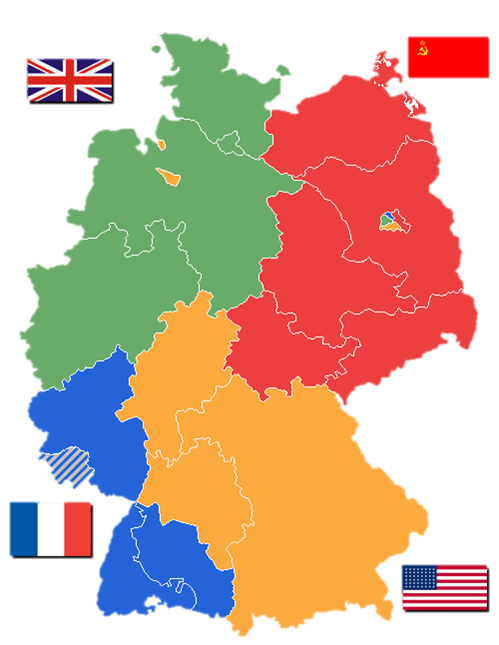
\includegraphics[width=250pt]{berlijn.png}
        \caption{Een geografische taart \ldots~ of misschien toch gewoon een kaart}
        \label{fig:berlijn}
    \end{center}
\end{figure}

\clearpage
\section{Bankroetproblemen}
\label{sec:bankroet}

Een bankroetprobleem is net als Fair Cake Cutting een verdeelprobleem. Het grote verschil is dat de spelers in een bankroetprobleem elk een eigen bedrag opeisen. Er is dus geen sprake meer van proportionaliteit. Bovendien wordt er geld verdeeld in plaats van stukjes taart, waardoor de spelers precies weten hoeveel zij hebben gekregen en het daar met elkaar niet oneens over zullen zijn. Het belangrijkste kenmerk van een bankroetprobleem is dat het bedrag dat de spelers samen eisen meer is dan het totaal te verdelen bedrag. Dit probleem kun je tegenkomen als iemand bankroet gaat en hij de spelers een bedrag verschuldigd is dat hij niet kan betalen. 

\subsection{De Talmud}
\setcounter{eis}{0}
Het bankroetprobleem was al bekend bij de Babyloni\"ers. In hun Talmud, een collectie van Joodse religieuze wetboeken die in de eerste vijf eeuwen na Christus op schrift is gesteld, is aan de hand van slechts drie voorbeelden beschreven hoe een eerlijke verdeling eruit zou zien:\\

\hspace*{\fill}\begin{minipage}{\textwidth-5mm}

    "Wanneer een man, die getrouwd is met drie vrouwen, overlijdt en hij heeft aan de eerste vrouw een schuld van 100 zuz, aan de tweede vrouw een schuld van 200 zuz en aan de derde vrouw een schuld van 300 zuz, en hij bezit bij zijn overlijden slechts 100 zuz, dan krijgt elk van de vrouwen een gelijk deel van dit bedrag.
    \ldots"\\
\end{minipage}

\noindent
In tabel \ref{tab:talmud} staat de volledige beschrijving van de oplossing in de Talmud samengevat. 

\begin{table}[htb]
  \centering
     \begin{tabular}{ c c | c c c | }
         \cline{3-5}
         && \multicolumn{3}{c |}{Nalatenschap} \\
         \cline{3-5}
	&&100&200&300 \\
         \cline{3-5}
         \hline
         \multirow{3}{1em}{\rotatebox{90}{Claim}} & 100 & 33,33 & 50 & 50 \\ 
         & 200 & 33,33 & 75 & 100\\
         & 300 & 33,33 & 75 & 150\\
         \hline
     \end{tabular}
  \caption{Zo moet je volgens de Talmud een nalatenschap van 100, 200 en 300 zuz verdelen.}
  \label{tab:talmud}
\end{table}

\subsection{Het betwiste-kleedprobleem}
We zien dat de eerste kolom gelijk verdeeld is, de derde kolom proportioneel verdeeld is en de tweede kolom ziet er raadselachtig uit. Uit een andere tekst uit de Talmud kon worden opgemaakt hoe je volgens hen een kleed moest verdelen onder twee spelers. Dit probleem met het kleed noemen we het betwiste-kleedprobleem of kortweg: \textbf{BK}.\\

\hspace*{\fill}\begin{minipage}{\textwidth-5mm}
    "Twee houden een kleed vast; de een claimt het hele kleed, de ander claimt de helft. Dan krijgt de een $\frac{3}{4}$, de ander $\frac{1}{4}$."\\
\end{minipage}

\begin{figure}[htb]
%  z = \overbrace{
%    \underbrace{x}_\text{real} +
%    \underbrace{iy}_\text{imaginary}
%   }^\text{complex number}
    \centering
    \resizebox{250pt}{!}{
    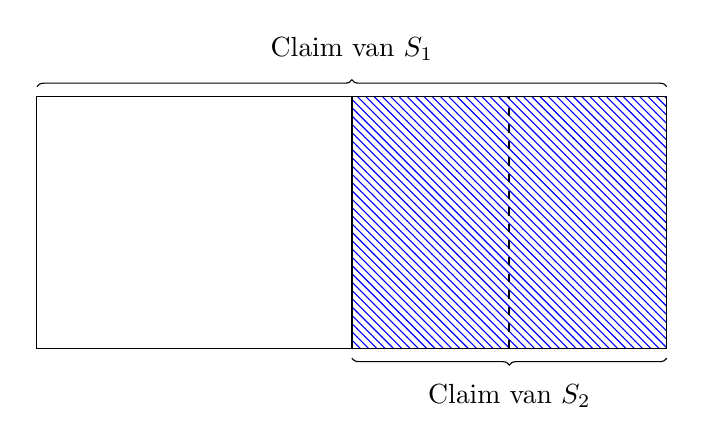
\begin{tikzpicture}
        \node (A) at (0,3.2){};
        \node (B) at (8,3.2){};
        \node(C) at (4,0){};
        \node (D) at (8,0){};
        \draw [decoration={brace}, decorate] (A.north) -- node[above=6pt] {Claim van $S_1$} (B.north);
        \draw (A) rectangle (D);
        \draw[pattern=north west lines, pattern color=blue] (B) rectangle (C);
        \draw[thick] (4,0) -- (4,3.2);
        \draw[thick,dashed] (6,0) -- (6,3.2);
        \draw [decoration={brace}, decorate] (D.south) -- node[below=6pt] {Claim van $S_2$} (C.south);
    \end{tikzpicture}
    }
    \caption{Illustratie van het betwiste-kleedprobleem}
    \label{fig:kleed}
\end{figure}

De gegeven oplossing door de Talmud valt te begrijpen aan de hand van figuur \ref{fig:kleed}. Hierbij claimt $S_2$ alleen de rechterhelft van het kleed. Om de linkerhelft wordt dus niet gevochten, dus die kunnen we alvast aan $S_1$ geven. Het deel van het kleed waar wel om gevochten wordt, verdelen we gelijk onder de spelers. Uiteindelijk krijgt $S_1$ op deze manier $\frac{3}{4}$ deel en $S_2$ $\frac{1}{4}$ deel, precies zoals de Talmud beschrijft. In het vervolg zullen we de claim van $S_i$ aanduiden met $C_i$. De totale waarde van het kleed of het totaal te verdelen bedrag, noemen we $K$.

%: Python oplossing voor 2 spelers
\label{subsec:AppOplossing_2}
\begin{lstlisting}
def BK_2(bedrag,claim_laag,claim_hoog):
    Error = is_bankroetprobleem(bedrag,claim_laag,claim_hoog)
    if Error:
        return Error
    speler_laag = max(0, bedrag - claim_hoog)
    speler_hoog = max(0, bedrag - claim_laag)
    
    # fifty-fifty de rest van het bedrag verdelen
    bedrag -= (speler_laag + speler_hoog)
    speler_laag += bedrag/2
    speler_hoog += bedrag/2

    # Noot: er is een unieke BK-oplossing
    return round(speler_laag,2), round(speler_hoog,2)
\end{lstlisting}

In Python, een programmeertaal, heb ik een functie geschreven die een de oplossing van een BK-probleem geeft op de genoemde manier. Eerst zal ik de basis uitleggen van Python, dit is belangrijk om alle volgende codes (gedeeltelijk) te begrijpen.
\begin{description}
\item [def] geeft aan dat er nu een functie volgt. De inhoud wordt pas uitgevoerd als de functie wordt aangeroepen. De functie roep je aan met de tekst die direct achter \verb|def| staat.
\item [return] geeft aan wat er teruggegeven moet worden als de functie aangeroepen wordt. Zodra de computer \verb|return| leest, stopt het uitvoeren van de functie ongeacht of er nog iets op latere regels staat.
\item [\#] geeft aan dat alles dat achter dit karakter op deze regel staat door de computer genegeerd moet worden.
\item [a = 5] betekent: neem variabele $a$ of maak een variabele genaamd $a$ aan als die nog niet bestond, en geef het de waarde 5.
\item [a += 2] is hetzelfde als \verb|a = a + 2|. Dus als $a$ eerst 5 was, dan is het na deze regel 7.
\item [round(a,b)] geeft het getal $a$ terug, afgerond op $b$ decimalen.
\item [n-tuple] is een geordende verzameling of lijst met $n$ elementen daarin.
\end{description}

\begin{figure}[htb]
    \begin{center}
        
\includegraphics[width=150pt]{machtig_python2.jpg}
        \caption{Machtig, dat Python}
        \label{fig:python1}
    \end{center}
\end{figure}

In regel 1 staat de syntax die de gebruiker moet gebruiken. Het eerste argument is het bedrag dat verdeeld dient te worden. Het tweede en derde argument zijn de laagste respectievelijk de hoogste claim. In het geval van het voorbeeld dat de Talmud beschrijft zou je dus \verb|BK_2(1,1,0.5)| moeten uitrekenen. Regels 2-4 zal ik later toelichten. In regel 5 wordt met \verb|bedrag - claim_hoog| het bedrag berekent waar de speler met de hoogste claim niet om zal vechten. Als die speler meer claimt dan het totale bedrag dat te verdelen valt, zou deze waarde negatief worden. Echter we laten de andere speler geen kleed inleveren om aan de behoefte te voldoen. Met \verb|max(0, bedrag - claim_hoog)| zorgen we ervoor dat alle negatieve waarden van \verb|bedrag - claim_hoog| vervangen worden door 0, dus de speler met de laagste claim niets hoeft in te leveren. Vervolgens maken we een variabele aan die de speler representeert en kennen we daar de waarde aan toe, d.w.z. het stuk kleed dat hij alvast krijgt. In regel 6 gebeurt hetzelfde, maar dan voor de andere speler. In regel 9 wordt berekent hoeveel kleed er nog over is om te verdelen. In regel 10 en 11 geven we beide spelers de helft van dit overige bedrag. In regel 14 geeft de functie uiteindelijk een 2-tuple terug met daarin de uitbetalingen aan de speler met de laagste claim respectievelijk de speler met de hoogste claim, afgerond in twee decimalen achter de komma.

Het blijkt dat in tabel \ref{tab:talmud} bij elk van de drie verschillende nalatenschappen geldt dat elk tweetal spelers BK-oplossingen zijn. Met andere woorden: $BK(X_i+X_j,C_i,C_j) = (X_i,X_j)$ voor elke combinatie $(i,j)$. \footnote{mits $S_i$ en $S_j$ gedefinieerd zijn.}

\subsection{De coalitionele procedure van Aumann en Maschler}
De wiskundigen Aumann en Maschler bewezen dat bovenstaande wiskundige regel ook geldt als je een speler door een coalitie zou vervangen, bijvoorbeeld $\{S_2\}$ vervangen door $\{S_2, S_3\}$. Dit wordt de coalitionele procedure van Aumann en Maschler genoemd. Om de oplossingen te vinden van een BK-probleem met meer dan twee spelers kunnen we dus als eerste argument het totaal te verdelen bedrag invullen, het tweede argument $C_1$ en als laatste argument de som van alle claims van de resterende spelers. Van de uitkomst die de functie teruggeeft, geven we $S_1$ zijn bedrag. Daarna herhalen we de functie recursief totdat iedereen het bedrag verdeelt is over alle spelers. Ik heb ervoor gekozen om een Python functie te schrijven die onafhankelijk van de functie voor twee spelers functioneert. Met onze kennis kunnen we de regels 5 tot en met 12 en regels 28 tot en met 37 begrijpen.\\

Ik zal eerst weer een paar gebuikte basisfuncties van Python uitleggen.
\begin{description}
\item [{[a,b]}] is de verzameling van de elementen a en b. \verb|[]| is een lege verzameling.
\item [if a: A, elif b: B, else: C] als $a$ een expressie is en waar is, doe dan handeling A. Als dat niet zo is, maar wel $b$ waar is, doe dan handeling B. Als niets van het vorige waar is, doe dan handeling C.
\item [for i in range(a,b)] geeft aan de code op de volgende regels, zolang die code begint met meer inspringing dan deze regel (die met \verb|for i in range(a,b)|), herhaald moet worden. Maak een variabele $i$ aan. De eerste keer is $i = a$. De tweede keer is $i = a + 1$, vervolgens $i = a + 2$, ... , en de laatste keer is $i = b -1$. Als je $a$ niet opgeeft, zal automatisch $a = 0$ worden genomen.
\item [function(a, *b)] De asterisk bij het tweede argument geeft aan dat we niet precies weten hoeveel argumenten we invoeren als we de functie gaan gebruiken. \verb|a| zal de waarde krijgen van ons eerste argument en \verb|b| zal een verzameling zijn van alle resterende argumenten. Dus \verb|function(1,2,3,4,5)| geeft als output \verb|a = 1, b = [2,3,4,5]|
\item [len(A)] is het aantal elementen in verzameling $A$, oftewel de \underline{len}gte van $A$.
\item [break] betekent: stop onmiddellijk met de \verb|for|-loop waar ik me nu in bevind.
\item [zip(A,B)] geeft een tuple van 2-tuples. Stel dat \verb|A = [1,2,3]| en \verb|B = [4,5,6]|. Dan is \verb|zip(A,B) = ( (1,4), (2,5), (3,6) )|
\item [OrderedDict] is een een soort van tuple van 2-tuples. Bijvoorbeeld: \verb|{a:1, b:2, c:3}|.
\end{description}

\begin{figure}[htb]
    \begin{center}
        
\includegraphics[width=150pt]{machtig_python.png}
        \caption{Het wordt me te machtig, dat Python!}
        \label{fig:python2}
    \end{center}
\end{figure}

%: Oplossing voor n spelers
\label{sec:AppOplossing_n}
\begin{lstlisting}
def BK(bedrag, *claims):
Error = is_bankroetprobleem(bedrag,*claims)
if Error:
    return Error
# komt neer op coalitionele procedure van Aumann en Maschler
from collections import OrderedDict
claims = sorted(list(claims))
subclaims = sum(claims)
coalitieomvang = len(claims)
result = []

for i in range(coalitieomvang - 1):
    subbedrag = min(claims[i],bedrag) / 2
    verlies = claims[i] - subbedrag
    # iemand met een lagere claim dient niet meer uitbetaald te krijgen dan iemand met een hogere claim
    if subbedrag >= bedrag/coalitieomvang:
        subbedrag = bedrag/coalitieomvang
        for _ in range(coalitieomvang):
            result.append(round(subbedrag,2))
        break
    # iemand met een lagere claim dient niet meer te verliezen dan iemand met een hogere claim
    elif (subclaims - coalitieomvang * verlies) < bedrag:
        verlies = (subclaims - bedrag) / coalitieomvang
        for j in range(coalitieomvang):
            result.append(round(claims[j] - verlies, 2))
        break
    else:
        result.append(round(subbedrag,2))
        bedrag -= subbedrag
    coalitieomvang -= 1
    subclaims -= claims[i]

# de laatste persoon krijgt de rest van het bedrag
result.append(round(bedrag,2))

#return result
return OrderedDict(zip(claims,result))
\end{lstlisting}

\myparagraph{Regels 5 tot en met 11: de initialisatie} 
Eerst komt de initilisatie, het aanmaken van variabelen. In regel 7 wordt de verzameling van alle claims, die we gegeven hebben als argument van de functie, gesorteerd van klein naar groot. In regel 8 maken we een variabele \verb|subclaims| aan dat de som van claims van alle spelers die nog in het spel zitten, aangeeft. Op dit moment zit iedereen nog in het spel. In regel 9 maken we een variabele \verb|coalitieomvang| aan die aangeeft hoeveel spelers er nog in het spel zitten. Verder maken we een verzameling \verb|result| aan die de uitbetalingen die we later gaan berekenen, opslaat.

\myparagraph{Regel 37: de return} 
Helemaal aan het einde, op regel 37, geeft de functie een verzameling terug met daarin 2-tuples. Het eerste element van de tuple is het geclaimde bedrag en het tweede element is de bijbehorende uitbetaling. Omdat we een \verb|OrderedDict| gebruiken, zullen de claims nog steeds van klein naar groot lopen als we de \verb|OrderedDict| op het scherm printen. Bovendien kunnen we met het commando \verb|OrderedDict[claim]| met \verb|claim| een van de claims in de verzameling \verb|claims| direct opvragen wat de bijbehorende uitbetaling is.

\myparagraph{Regels 12, 13, 30, 31 en 34: het eigenlijke verdeelproces} 
\label{subbedrag}
Na de initialisatie, komt het rekenwerk. Met \verb|for i in range(coalitieomvang - 1)| doorlopen we met variabele \verb|i| alle spelers, behalve de laatste speler. Hij krijgt het bedrag dat over is als alle anderen hun uitbetaling gekregen hebben, zie regel 34. In regel 13 wordt een variabele \verb|subbedrag| gemaakt met de uitbetaling die $S_i$\footnote{Deze $i$ is dezelfde i als de i van de for-loop.} zou moeten krijgen. Deze regel is goed te begrijpen aan de hand van figuur \ref{fig:kleed}. Stel je even voor dat wij de computer zijn en bij regel 13 van de code zijn aanbeland. 

Stel dat $C_i \geq K$. Dan is $S_1 \neq S_n$, want als dat zo zou zijn, dan zouden we niet bij de \verb|for|-loop op regel 13 kunnen zijn. Immers de laatste speler krijgt zijn uitbetaling in regel 34. Er is dus minstens \'e\'en speler na $S_i$, noem hem $S_{i+1}$. Bovendien is $C_{i+1} \geq C_i \geq K$. Dus er is geen stuk kleed waar niet om gevochten wordt. Daarom wordt $K$ gelijk verdeeld onder $S_i$ en de verzameling van alle andere spelers die nog in het spel zitten. Dus $X_i = \frac{K}{2}$.

Stel nu dat $C_i < K$. $S_1$ krijg in elk geval $\frac{1}{2} \cdot C_i$ uitbetaald.. Het kan het zijn dat $C_{i+1} \geq C_i < K$. Omdat $S_{i+1}$ wel eens de enige speler zou kunnen zijn die nog in het spel zit en ongelijk is aan $S_i$ zelf, kan het dus zijn dat de claim van die coalitie gelijk is aan $C_{i+1} \geq C_i < K$. In dat geval krijgt $S_i$ nog een extra bedrag. Echter dit wordt nog niet rechtgezet in regel 13, maar in regels 22 tot en met 26.

\myparagraph{Regels 15 tot en met 20: de maximale uitbetaling}
\label{aanvullende_eigenschap1}
Het is redelijk om te stellen dat een speler die minder claimt, ook minder uitbetaald krijgt. Voor zover we de Python code hebben bekeken gaat het fout bij \verb|BK(300,300,400,500)| $\rightarrow$ \verb|{300: 150.0, 400: 150.0, 500: 0.0}|. Als we dus een bedrag willen uitbetalen aan een speler, maar het blijkt dat er dan te weinig meeer overblijft van het totaalbedrag om minimaal dezelfde uitbetaling te geven aan elk van de andere spelers die nog in het spel zitten, dan stoppen we met berekenen en geven we elke speler die nog in het spel zit een gelijk bedrag. Dit is precies wat er gebeurt in de regels 15 tot en met 20 van de Python functie.

\myparagraph{Het maximale verlies}
Een speler met een lagere claim dient niet meer te verliezen dan een speler met een hogere claim. Als bijvoorbeeld $C_1 = 50$ en $X_1 = 20$, dan is zijn verlies $50-20=30$. De aanvullende eigenschap valt te verdedigen, maar is al minder triviaal dan de eigenschap in de vorige paragraaf. Echter we hebben ook nog iets recht te zetten in regel 13, omdat we de BK-procedure voor twee personen niet volledig hebben uitgevoerd. Laten we namelijk \verb|BK(100,50,51)| uitrekenen, dan krijgen we het resultaat \verb|{50: 25.0, 51: 75.0}| en dat is duidelijk niet eerlijk. Dit probleem wordt direct opgelost als we de aanvullende eigenschap programmeren, Immers in het voorbeeld is $V_1 = 25.0 > -25.0 = V_2$ waarbij $V_i$ even het verlies voor speler i aangeeft. 

\myparagraph{Regels 21 tot en met 26: maximaal verlies}
Regel 22 begint, op de inspringing na, met het commando \verb|elif|. Merk op dat dit nu hetzelfde effect heeft als \verb|if|, omdat de computer alleen bij regel 22 aanbeland kan zijn als het \verb|if|-statement op regel 16 onwaar is en dus het bijbehorende \verb|break| commando niet is uitgevoerd. Om te controleren of $S_i$ een groter verlies heeft dan een van de spelers met een hogere claim dan hij (dat zijn precies alle andere spelers die nog in het spel zitten en dat zijn \verb|subclaim| spelers), gaan we na of er een bedrag overblijft als we alle spelers met een hogere claim hetzelfde verlies geven als dat van $S_i$. Als dat namelijk gebeurt, dan moeten we een of meerdere spelers met een hogere claim een (deel van) het resterende, te verdelen bedrag geven, waardoor zijn (of hun) verlies kleiner wordt dan dat van $S_i$. De werking van de Python code in regels 23 tot en met 26 is equivalent aan die van regels 17 tot en met 20.

%%\subsubsection{Anonimiteit}
%%Merk op dat we geen variabelen hebben voor de spelers. Dit komt omdat de enige eigenschap van een speler de hoogte van zijn claim is. Het zou niet mogen uitmaken of een willekeurige speler, zeg Gerrit, die altijd 40 zuz claimt, $S_1$ of $S_2$ wordt genoemd.\\
%%
%%\begin{eis}{\textbf{Anonimiteit}: het zou niet mogen uitmaken hoe een bepaalde speler wordt genoemd.} \end{eis}

%%\subsubsection{Communicerende vaten}

\subsection{Verder Python onderzoek}
Als je genoten hebt van de Python functies, dan wijs ik je graag op bijlage \ref{sec:AppBankroet} en bijlage \ref{sec:AppCooperatief}, want daar staan nog veel meer leuke Python functies die te maken hebben met speltheorie!

%%\subsection{Verdelen met behulp van de co\"operatieve speltheorie}
%%\subsubsection{De core van een spel}
%%
%%%: 3D assenstelsel naar vlak
%%\begin{tikzpicture}[->,scale=2]
%%\draw (0,0) -- (2.5,0,0) node [right] {$x$};
%%\draw (0,0) -- (0,2.5,0) node [above] {$y$};
%%\draw (0,0) -- (0,0,2.5) node [below left] {$z$};
%%\draw[red,thick] (0,0,1) node[shade,top color=white,anchor=north] {$(0,0,10)$}
%%    -- (0,1,0) node[shade,top color=white,draw=none,anchor=south] {$(0,10,0)$}
%%    -- (1,0,0) node[shade,top color=white,anchor=west] {$(10,0,0)$}
%%    -- cycle;
%%\end{tikzpicture}
%%
%%\subsubsection{De nucleolus}
%%\subsubsection{De Shapley-waarde}

% ----------------------------------------------------------------------------------------------------------------------------------

%%\color{red}
%%\clearpage
%%\section{Huwelijksproblemen}
%%wat zijn huwelijksproblemen
%%
%%\subsection{Wat is een huwelijksprobleem}
%%\subsection{De stelling van Hall}
%% blind kwartet als voorbeeld
%%\subsection{Het huwelijksprobleem met preferenties}
%%
%%\clearpage
%%\section{Optimaal Stoppen}
%%[wat is het] en [het belang]
%%
%%politie / googols spel (martin gardner) / secretaresseprobleem (merrill m. flood)
%%
%%varianten
%%
%%experimenteel onderzoek
%%
%%\clearpage
%%\section{Beroemde dilemma's}
%%\subsection{Het Prisoners' Dilemma}
%%nash-evenwicht
%%\subsection{Centipede Game}
%%\subsection{Battle of the Sexes}
%%\subsection{Twee derde van het gemiddelde}
%%\color{black}

\clearpage
\section{Politieke kiessystemen: perfecte democratie is onmogelijk}
\label{sec:democratie}

\begin{wrapfigure}{r}{0cm}
    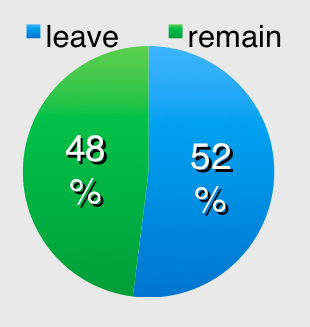
\includegraphics[width=100pt]{britten_uitslag.png}
    \label{fig:CoreDrawVB}
\end{wrapfigure}
In de vroege ochtend van 24 juni 2016 werd bekend gemaakt dat het Verenigd Koninkrijk middels een referendum had besloten om de Europese Unie te verlaten. Immers 52\% van de opkomst en dus de meerderheid van bevolking stemde voor 'leave'. Al de volgende dag had dat negatieve gevolgen voor Europese landen, in het bijzonder voor de Britten zelf. De financi\"ele markt stortte in, net zo abrupt als de val van een kaartenhuis. 
\begin{wrapfigure}{l}{0cm}
    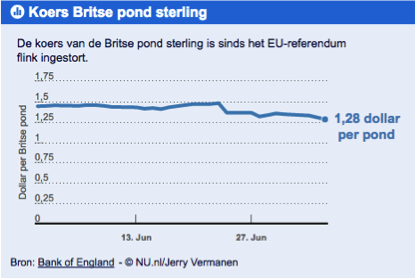
\includegraphics[width=200pt]{pond_daling.png}
    \label{fig:CoreDrawVB}
\end{wrapfigure}
De pond daalde op de bewuste dag maar liefst 8\% in waarde en bleef zakken tot een dieptepunt van 1,28 doller per pond op 6 juli. Londen is niet langer meer het financi\"ele centrum van Europa, waardoor het toekomstperspectief er voor de Britten slecht uit ziet. Verschillende banken verloren een vijfde van hun beurswaarde en zelfs Britse parlementsleden met inbegrip van de premier kondigden massaal hun vertrek aan. Logischerwijs gaan er stemmen op om opnieuw te gaan stemmen. De petitie was ondersteund door miljoenen handtekeningen, maar werd afgeslagen door de premier.

Het is niet de eerste keer dat een referendum resulteert in een controverse. Eerder waren het bijvoorbeeld de Schotten die met 55\% tegen onafhankelijkheid stemden en onze eigen Associatieovereenkomst met een ietwat overtuigender afkeuring van 61\%.

In Nederland zijn we gewend aan het 'meeste stemmen gelden' -systeem, omdat dat  ook wordt gebruikt in de politiek. Er is dus geen ruimte  voor een tweede keuze. Het gevolg is dat je als kiezer simpelweg de grootste achterban moet vormen. Stel dat school jou een enqu�te laat invullen met de vraag welk elektronisch hulpmiddel ze zouden moeten invoeren. Het liefst zou je de MacBook willen, op de tweede plek staat de iPad en van de Windows laptop walg je. Met het vermoeden dat de MacBook geen grote achterban zal hebben, is het verstandiger om de iPad als eerste keuze op te geven, terwijl het eigenlijk je tweede keuze is. Dat wordt strategisch stemmen genoemd.

\begin{figure}[b]
    \centering
    \begin{minipage}{.5\textwidth}
          \centering
          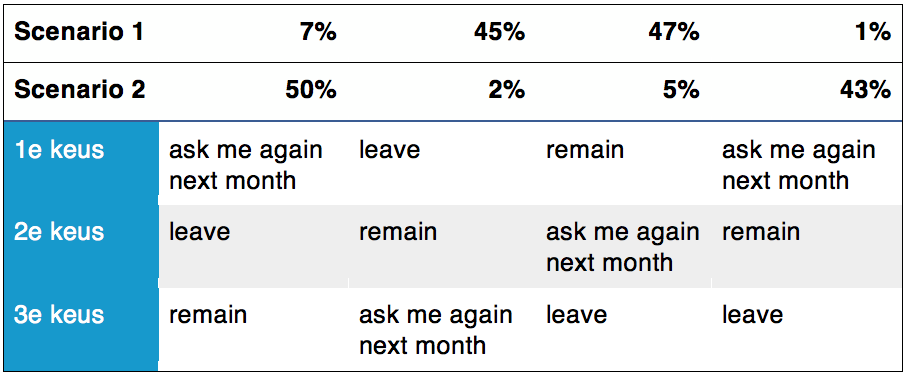
\includegraphics[width=.9\linewidth]{britten2.png}
          \label{britten1}
    \end{minipage}%
    \begin{minipage}{.5\textwidth}
          \centering
          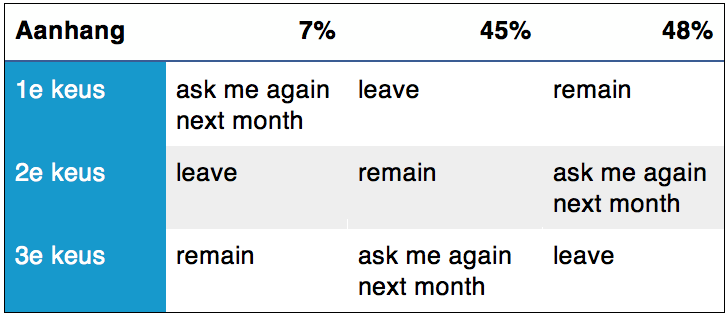
\includegraphics[width=.9\linewidth]{britten1.png}
          \label{britten2}
    \end{minipage}
\end{figure}

Natuurlijk kun je op dezelfde wijze de gebreken in het systeem misbruiken. Dan heet het fraude. Cameron zou als aanhanger van 'remain' bijvoorbeeld naast 'remain' en 'leave' een derde keuzemogelijkheid 'ask again next month' kunnen toevoegen, terwijl hij twee dingen weet. Ten eerste heeft het leave camp meer de wens om nog eens over hun keuze na te denken dan het remain camp. Ten tweede heeft iemand hem onder vier ogen verteld dat het binnenkort duidelijk wordt dat er geen tijd is om langer na te denken. De wensen van het volk zijn verdeeld zoals in de tabel. Zou men enkel naar de eerste keuze kijken, dan wint het remain camp met een nipte meerderheid volgens de verdeling in het eerste scenario. Ook in het tweede scenario wint het remain camp, maar pas nadat de EU het Britse volk bekend maakt dat de Britse regering snel een keuze moet maken. Daardoor valt de keuzemogelijkheid 'ask me again next month' af, ondanks het feit dat 93\% van de Britten voor die keuze stond.

\begin{wrapfigure}{l}{0cm}
    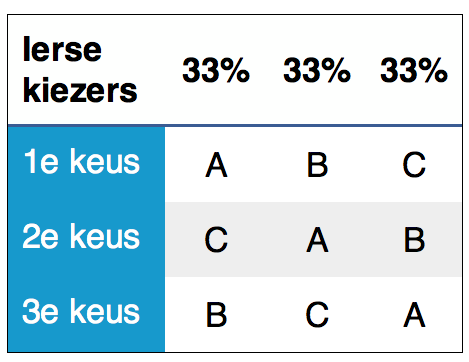
\includegraphics[width=120pt]{verkiezing_ieren.png}
    \label{fig:CoreDrawVB}
\end{wrapfigure}

Nu zul je je misschien afvragen waarom dit kiessysteem heersend is in Nederland, want het blijkt nare bijverschijnselen te vertonen bij de analyse en veel buurlanden gebruiken andere systemen. In Frankrijk wordt bijvoorbeeld de tweede keuze nog meegenomen in politieke beslissingen, wat al flink genuanceerder lijkt dan het Nederlandse systeem. In Ierland kun je een compleet lijstje van je voorkeuren doorgeven en tot slot is er Noord-Korea waar hypothetische eerste keuzes direct de prullenmand in gaan. 

Het lek van het Ierse systeem is dat er niet altijd een uitslag is. In de tabel hiernaast bijvoorbeeld is het volstrekt duidelijk dat drie keuzemogelijkheden A, B en C even gewenst zijn als respectievelijk eerste -, tweede - en derde keuze. Ook is er geen uitslag als je de wensen per groep kiezers bekijkt. Elke groep vertegenwoordigt $\frac{1}{3}$ van de bevolking en tellen dus even zwaar mee in het Ierse systeem. $\frac{2}{3}$ van de bevolking verkiest keuze A boven keuze B, evenals $\frac{2}{3}$  van de bevolking die B boven C kiest. Logischerwijs zou A dus veel gewenster moeten zijn dan C, maar niets is minder waar: ook $\frac{2}{3}$  van de bevolking verkiest C boven A. Kortom elke keuze is gewenster dan de twee andere keuzes, maar dat kan natuurlijk niet leiden tot een redelijk besluit.

Er zijn nog veel meer mogelijke kiessystemen in omloop. Bijvoorbeeld het eliminatiesysteem dat Expeditie Robinson, Voice of Holland of een willekeurig ander televisieprogramma toepast. Het stemmen duurt hier extreem lang, waardoor het meerdere afleveringen in beslag neemt en dus leidt tot meer inkomsten voor de programmamakers. Dit is tevens het nadeel op politiek niveau. 

In Amerika wordt er gestemd per regio of deelstaat. Enkel de eerste keuze van alle mensen binnen een bepaalde deelstaat wordt meegenomen naar de gezamenlijke besluitvorming van alle deelstaten. Vervolgens heeft elke deelstaat dus een weging en een voorkeur. Ten slotte wordt deF uit die verzameling eerste keuzes van deelstaten een eerste keuze van de staat bepaald. Dit systeem nodigt op het eerste gezicht uit om tot paradoxale uitslagen te komen. Anderzijds is het uniek, omdat geen enkel ander politiek systeem be�nvloed wordt door geografische factoren. In het geval van het EU-referendum van het Verenigd Koninkrijk zou dit aspect met gemak een heel ander eindresultaat opleveren. In Londen en in heel Schotland stemde men bijvoorbeeld 75\% voor 'remain' en 25\% voor 'leave'. Buiten de grote steden waren de rollen omgekeerd.

Tot slot heeft het Verenigd Koninkrijk net als veel andere landen het aspect dat er een minimum percentage van de bevolking moet stemmen om de uitslag geldig te mogen verklaren. Dit wordt het opkomstpercentage genoemd. Het resulteert in de beroemde 'was ik nou maar thuis gebleven'- paradox. Het komt erop neer dat een groep mensen die in de minderheid zijn en voor A stemmen juist door te stemmen B waarmaken, terwijl A de uitslag zou zijn geweest als ze helemaal niet hadden gestemd. Dit is natuurlijk een ongewenst effect van het kiessysteem met een voorwaarde van opkomstpercentage.
 
Wiskundig gezien bestaat er geen perfect kiessysteem, want elk kiessysteem vertoont zijn eigen paradoxen. Kenneth Arrow bewees dit en ontving daarvoor de Nobelprijs voor de Economie in 1972. Er zijn nog vele andere boeken over dit onderwerp geschreven, zowel voor parlementari\"ers als wiskundigen en scholieren.

%%\color{red}
%%\clearpage
%%\section{Vormen van weergave}
%%normaal, extensief, matrix, spelboom, Nim verloren inzicht
%%	NIM: spiegelstrategie, reduceren probleem
%%		Reduceren: recursief algoritme, symmetrie, onvermijdelijke sets, backward induction, samennemen van opties
%%
%%\clearpage
%%\section{De Sonttol: een toepassing}
%%\color{black}

\clearpage
\section{Samenvatting}
De speltheorie is een erg breed discipline. Het verdelen van een deelbaar goed, waarbij rationele spelers over mening kunnen verschillen over de waarde van delen van het goed, blijkt een moeilijke opgave te zijn. Er zijn sinds het ontstaan van de speltheorie in de twintigste eeuw tientallen verschillende protocollen opgesteld. Echter de ultieme oplossing, een proportioneel, jaloezie-vrij protocol met lage complexiteit, is vandaag de dag niet gevonden. We hebben gezien dat als er een dergelijk protocol bestaat, dat de complexiteit ervan maximaal $n\aesuper[1]{n\aesuper{n\aesuper{n\aesuper{n\aesuper{n}}}}}$ is.

Erfenissen laten zich iets gemakkelijker verdelen, omdat de waarde ervan uit te drukken is in geld. Hierdoor weten alle spelers precies wat ze hebben gekregen en wat de andere spelers hebben gekregen. Toch zijn er ook hier verschillende opvattingen over wat eerlijk is. De nucleolus en de Shapley-waarde zijn twee verschillende oplossingen met veel aanhang.

%%Het vormen van koppels tussen een groep (heteroseksuele) mannen en -vrouwen is een huwelijksprobleem. Een meer gangbare toepassing wordt duidelijk als men studenten met universiteiten koppelt in plaats van mannen met vrouwen. De stelling van Hall geeft een methode om makkelijk na te gaan of een huwelijksprobleem oplosbaar is.
%%
%%Optimaal stoppen is een spelsoort waarbij men (de kans op) winst kan maximaliseren door het moment van beslissing te bepalen. Bedrijven moeten bijvoorbeeld vaak overwegen hoelang ze doorgaan met het ontwikkelen van een product en dus hoe lang ze zullen wachten met het uitbrengen ervan op de markt. Hoe langer het product ontwikkeld wordt, hoe beter het product wordt en de tevredenheid van de klant stijgt. Echter geldt ook dat men de concurrent voor moet blijven. Tussen de twee uitersten zal een punt liggen waarbij de verwachte winst optimaal is. 

Tot slot hebben we gezien dat politieke kiessystemen ook slecht oplosbaar zijn en dat bepaalde combinaties van wensen zelfs onmogelijk blijken te zijn.

\clearpage
\section{Conclusie}
Voor de analyse van spellen zijn bepaalde aannames gedaan, die lang niet altijd overeenkomen met de werkelijkheid. In de re\"ele wereld willen we elkaar doorgaans namelijk dingen gunnen en doen we niet moeilijk over een gram taart te weinig. Bovendien zal de mens altijd tegen het probleem blijven lopen dat voorkeuren moeilijk uit te drukken zijn in getallen en bovendien afhankelijk is van tijd. Tot slot moet de werkelijkheid vaak sterk versimpeld worden, omdat de speltheorie slechts een beperkt aantal stellingen heeft.\footnote{In wiskundige zin zal dit ook altijd "beperkt" blijven} Maar de speltheorie is nog jong, dus misschien moeten we haar gewoon wat extra tijd gunnen.

\clearpage
\section{Bijlagen}
\appendix{}

%: Bijlage Recursiviteit
\section{Recursiviteit}
\label{sec:AppRecursief}
Er staan n stoelen op een rij en op elke stoel zit een persoon. Iedereen staat op en neemt daarna weer plaats, al dan niet op een andere stoel. Het blijkt dat elke persoon maximaal \'e\'en stoel opgeschoven is. Op hoeveel manieren kan dit bereikt worden?

\begin{figure}[htb]
    \centering
     \resizebox {\linewidth}{!}{
            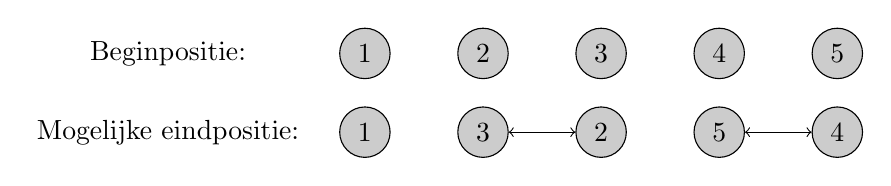
\begin{tikzpicture}[mystyle/.style={circle,draw,fill=gray!40,inner sep=0pt,text width=6mm,align=center}]
      \node (-1) at (-1,1) {Beginpositie:};
      \node (0) at (-1,0) {Mogelijke eindpositie:};
      \node [mystyle]  (1) at (1.5*1,0) {1};
      \node [mystyle]  (2) at (1.5*2,0) {3};
      \node [mystyle]  (3) at (1.5*3,0) {2};
      \node [mystyle]  (4) at (1.5*4,0) {5};
      \node [mystyle]  (5) at (1.5*5,0) {4};
      \draw [<->] (4) -- (5);
      \draw [<->] (2) -- (3);
      \foreach \x in {1,...,5}
%           {\pgfmathtruncatemacro{\label}{\x}
       {\node [mystyle]  (\x,1) at (1.5*\x,1) {\x};}
            \end{tikzpicture}
            }
    \caption{Illustratie van het raadsel}
    \label{fig:additief}
\end{figure}
\noindent
{\textcolor{red}{\textbf{Let op: hierna volgt het antwoord en de uitwerking}}
\\[.8in]
\noindent
\paragraph{Antwoord}
het $n^{de}$ fibonacci-getal. 
\paragraph{Uitwerking}
Stel  er zijn $k = n$ stoelen. Een persoon kan alleen van plek wisselen met zijn of haar buurman. Stel dat de persoon op stoel $k$ niet wisselt met zijn linkerbuurman, dan kunnen we deze $k^{de}$ persoon vergeten. Immers niemand anders dan de linkerbuurman kan interactie met deze persoon hebben. Het antwoord is dus hetzelfde als dat bij $k = n-1$. Stel nu dat de persoon op stoel $k$ wel wisselt met zijn linkerbuurman, dan kunnen we de $k^{de}$ en $k-1^{de}$ persoon vergeten. Immers niemand anders kan nog interactie met deze twee personen hebben. Het antwoord is dus hetzelfde als dat bij $k  = n-2$. Deze twee gevallen bij elkaar optellen geeft $f(k) = f(k-1) + f(k-2)$ waarbij $f(k)$ het aantal manieren om van plek te wisselen geeft bij $k$ stoelen. Bovendien geldt $f(0) = 1 = F(0)$ en $f(1) = 1 = F(1)$ waarbij $F(n)$ het $n^{de}$ fibonacci-getal geeft. Dus $f(n) = F(n)$.
\paragraph{Wat hebben we geleerd?}
Soms is het handig of zelfs noodzakelijk om recursie te gebruiken bij het opstellen van een formule f(n). Dat wil zeggen dat we een triviaal antwoord gebruiken, meestal $n = k = 0$ of $n = k = 1$, in combinatie met een formule om $f(k+1)$ om te schrijven in $f(k)$.

%: Bankroet
\newpage
\section{Bankroet met Python}
\label{sec:AppBankroet}

%: Is het een bankroetprobleem?
\label{subsec:Appis_bankroet}
\subsection*{Is het een bankroetprobleem?}
\begin{lstlisting}
def is_bankroetprobleem(bedrag, *claims):
    if False in [x >= 0 for x in claims]:
        return 'Error: negatieve argumenten ingevoerd'
    if sum(claims) < bedrag:
        return 'Error: het bedrag is groter dan de totale claim'
\end{lstlisting}

%: Controleer de oplossing
\label{sec:AppControle}
\subsection*{Controleer de oplossing}
\begin{lstlisting}
def is_BK_consistent(dict):
    # controleert of een verdeling van claims en uitbetalingen BK-consistent is
    from itertools import combinations
    bedrag = sum(dict.values())
    paren = combinations(dict.keys(),2)
    for x in paren:
        A = dict[x[0]]
        B = dict[x[1]]
        if not BK_2(A+B, x[0], x[1]) == (A, B):
            return False
    return True
\end{lstlisting}

\section{Co\"operatieve spellen}
\label{sec:AppCooperatief}

%: Nucleolus berekenen
\label{sec:AppNucleolus}
\subsection*{Bereken de nucleolus van een cooperatief spel}
\begin{lstlisting}
def nucleolus(N, *waarden):
    waarden = list(waarden)
    from itertools import combinations
    from math import factorial
    spelers = list(range(1,N+1))
    coalities = [list(x) for i in range(N+1) for x in combinations(spelers,i)]
    a = waarden[-1] - sum([waarden[i] for i in spelers])
    while a > 0:
##        print(a)
        speling = []
        for i in spelers:
            list_substract = coalities[2**N - i - 1]
            speling.append( (waarden[-1] - waarden[coalities.index(list_substract)]) - (waarden[i]) )
        spelers = [spelers[x] for x in range(len(spelers)) if speling[x] != 0]
        speling = [x for x in speling if x != 0]
        translatie = min(a / len(spelers), .5 * min(speling) )
##        print(speling, a / len(spelers))
##        print(translatie)
##        print(spelers)
        for i in spelers:
            waarden[i] += translatie
            waarden[2**N - i - 1] += translatie
##        print(waarden)
        a = waarden[-1] - sum([waarden[i] for i in range(1,N+1)])
    #return [round(x,3) for x in waarden[1:N+1]]
    return waarden
\end{lstlisting}

%: Shapley waarde berekenen
\label{sec:AppShapley}
\subsection*{Bereken de shapley waarde van een cooperatief spel}
\begin{lstlisting}
def Shapley(N, *waarden):
    from itertools import combinations
    from math import factorial
    coalities = [list(x) for i in range(N+1) for x in combinations(range(1,N+1),i)]
    teller = [factorial(len(x)) * factorial(N - len(x) - 1) for x in coalities if not 1 in x]
    noemer = factorial(N)
    sommatie = [[x for x in coalities if i not in x] for i in range(1,N+1)]
    result = []
    for i in range(1,N + 1):
        shapley = 0
        for j in range(len(teller)):
            shapley += (teller[j] * ( waarden[coalities.index(sorted(sommatie[i-1][j] + [i] ))] - waarden[coalities.index(sommatie[i-1][j])] ))
        result.append(round(shapley/noemer, 3))
    return result
\end{lstlisting}

%: CoreDraw voorbeeld
\label{sec:AppCoreDrawVB}
\subsection*{Voorbeeld van de functie CoreDraw, geschreven in Python}

\begin{figure}[htb]
    \centering
    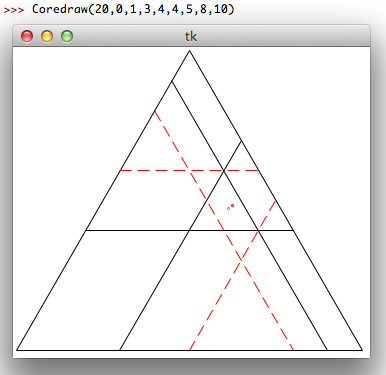
\includegraphics[width=200pt]{coredraw_voorbeeld.png}
    \caption{Voorbeeld van de functie CoreDraw in Python op ee}
    \label{fig:CoreDrawVB}
\end{figure}

%: CoreDraw
\label{AppCoreDraw}
\subsection*{Teken de core met {\color{red}shapley-waarde} en{ \color{green}nucleolus}.}
\begin{lstlisting}
def Coredraw(scale_method, *waarden):
    "0 voor gelijk houden; null; 1; 2; 3; 1,2; 1,3; 2,3'"
    #translatie (.5 ; .5), dus middelpunt gelijkzijdige driehoek
    if scale_method == 0:
        scale = 300 / waarden[7]
    else:
        scale = scale_method

    import tkinter as tk
    root = tk.Tk()
    width_ = waarden[7] * 3**.5 * scale + 5
    height_ = 1.5 * waarden[7] * scale + 5
    w = tk.Canvas(root, width = width_, height = height_)
    w.pack()
    ez = (0, -scale)
    ey = (.5 * scale * 3**.5, .5 * scale)
    ex = (-.5 * scale * 3**.5, .5 * scale)

    def drawline(coords1, coords2, **kwargs):
        w.create_line(.5 * width_ + coords1[0] * ex[0] + coords1[1] * ey[0] + coords1[2] * ez[0],
                     2/3 * height_ + coords1[0] * ex[1] + coords1[1] * ey[1] + coords1[2] * ez[1],
                     .5 * width_ + coords2[0] * ex[0] + coords2[1] * ey[0] + coords2[2] * ez[0],
                     2/3 * height_ + coords2[0] * ex[1] + coords2[1] * ey[1] + coords2[2] * ez[1],
                     **kwargs)
                     
    drawline( (0,0,waarden[7]), (0,waarden[7],0) )
    drawline( (waarden[1],0,waarden[7] - waarden[1]), (waarden[1], waarden[7] - waarden[1], 0) )
    drawline( (waarden[7] - waarden[6], 0, waarden[6]), (waarden[7] - waarden[6], waarden[6], 0), dash=(12,6), fill='red' )

    drawline( (0,0,waarden[7]), (waarden[7],0,0) )
    drawline( (0, waarden[2], waarden[7] - waarden[2]), (waarden[7] - waarden[2], waarden[2], 0) )
    drawline( (0,waarden[7] - waarden[5], waarden[5]), (waarden[5], waarden[7] - waarden[5], 0), dash=(12,6), fill='red' )

    drawline( (waarden[7],0,0), (0,waarden[7],0) )
    drawline( (waarden[7] - waarden[3],0,waarden[3]), (0,waarden[7] - waarden[3],waarden[3]) )
    drawline( (waarden[4], 0, waarden[7] - waarden[4]), (0, waarden[4], waarden[7] - waarden[4]), dash=(12,6), fill='red' )
    
    def drawcircle(coords1, **kwargs):
        x = .5 * width_ + coords1[0] * ex[0] + coords1[1] * ey[0] + coords1[2] * ez[0]
        y = 2/3 * height_ + coords1[0] * ex[1] + coords1[1] * ey[1] + coords1[2] * ez[1]
        w.create_oval(x-1, y-1, x+1, y+1, **kwargs)
    drawcircle(tuple(Shapley(3,*waarden)),outline='red')
    drawcircle(nucleolus(3,*waarden)[1:4],outline='green')
    
    tk.mainloop()
\end{lstlisting}

\section{Huwelijksproblemen}

%: Preferentie huwelijksprobleem
\label{sec:AppHuwelijk1}
\subsection{Preferentie huwelijksproblemen oplossen}
\begin{lstlisting}
def preferentie_huwerlijksprobleem(wensen_mannen, wensen_vrouwen):
    "Geordende lijst zonder weigeren passieve vrouwen\nVB: {'a':'cd', 'b':'dc'}, {'c':'b','d':'a'}"
    koppels = {}
    preferentie = {}
    for man in wensen_mannen:
        preferentie[man] = 0
    for man in wensen_mannen.keys():
        if not man in koppels.keys():
            while True:
                try:
                    aangevraagde = wensen_mannen[man][preferentie[man]]
                except IndexError:
                    del koppels['b']
                    break
##                print('ask ', man, aangevraagde)
                if not aangevraagde in koppels.values():
                    koppels[man] = aangevraagde
##                    print('init ', man, aangevraagde)
                    break
                else:
                    bruiloft = False
                    for prefer_vrouw in wensen_vrouwen[aangevraagde]:
                        if prefer_vrouw == man:
                            koppels[man] = aangevraagde
                            bruiloft = True
                            continue
                        elif not prefer_vrouw in koppels.keys():
                            continue
                        elif koppels[prefer_vrouw] == aangevraagde:
                            if bruiloft == False:
##                                print('verloren van ',prefer_vrouw)
                                pass
                            else:
##                                print('gewonnen van ',prefer_vrouw)
                                man = prefer_vrouw
                            preferentie[man] += 1
                            break
    return koppels
\end{lstlisting}

\clearpage
\begin{thebibliography}{1}

\section*{Boeken}
  \bibitem{recreational}  \textsc{Averbach, B., \& Chein, O.} (1999). {\em Problem Solving Through Recreational Mathematics}. Dover Books
  \bibitem{kwartet}  \textsc{Brakenhoff, J., \& Stolk A.} (2015). {\em Blind Kwartetten}. Vierkant voor Wiskunde
  \bibitem{inleiding}  \textsc{Davis, M. D.} (1973). {\em Inleiding tot de speltheorie}. Utrecht/Antwerpen: Het Spectrum B. V.
  \bibitem{zebra}  \textsc{Thuijsman, F.} (2005). {\em Spelen en Delen: Speltheorie, de wiskunde van conflictmodellen}. Utrecht: Epsilon Uitgaven

  \section*{Krantenartikelen}
  \bibitem{protocollen2}  \textsc{Brams, S. J., \& Taylor, A. D.} (1995, januari). {\em An Envy-Free Cake Division Protocol}. The American Mathematical Monthly, Vol. 102, No. 1, (Jan., 1995), pp. 9-18

\section*{Websites}
  \bibitem{selfridge}  \textsc{Carnegie Mellon University}, (2012, 7 juni). {\em 15-451 Algorithms}.  Geraadpleegd op 18 december 2016, van http://www.cs.cmu.edu/afs/cs/academic/class/15451-f07/www/lectures/lect1206.txt

  \bibitem{protocollen_beamer}  \textsc{Endriss, U.} (2013). {\em Computational Social Choice: Autumn 2013}.  Geraadpleegd op 18 december 2016, van https://staff.science.uva.nl/u.endriss/teaching/comsoc/2013/slides/comsoc-cakes.pdf
  
  \bibitem{optimaal_stoppen}  \textsc{Hill T.,} (2009, april). {\em Knowing When to Stop: How to gamble if you must?the mathematics of optimal stopping}.  Geraadpleegd op 18 december 2016, van http://www.americanscientist.org/issues/feature/2009/2/knowing-when-to-stop/1
  
  \bibitem{kankerbestrijding}  \textsc{Kianercy, A., Veltri, R., \& Pienta, K. J.}., (2014, 20 juni). {\em Critical transitions in a game theoretic model of tumour metabolism}.  Geraadpleegd op 18 december 2016, van http://rsfs.royalsocietypublishing.org/content/4/4/20140014.full

   \bibitem{texample_tree}  \textsc{Kirsch, M.} (2009, 16 december). {\em Example: Merge sort recursion tree}.  Gedownload op 18 december 2016, van http://www.texample.net/tikz/examples/merge-sort-recursion-tree/

   \bibitem{latex_tutorial}  \textsc{latex-tutorial.com} (2015, 13 oktober). {\em A simple guide to LaTeX: Step by Step}.  Geraadpleegd op 18 december 2016, van https://www.latex-tutorial.com/tutorials/

   \bibitem{effbot}  \textsc{Lundh, F.} (z.d.). {\em The Tkinter Canvas Widget}.  Gedownload op 18 december 2016, van http://effbot.org/tkinterbook/canvas.htm

  \bibitem{math_alive}  \textsc{Math Alive, S.} (2006, 26 april). {\em Voting and Social Choice}.  Geraadpleegd op 18 december 2016, van http://web.math.princeton.edu/math\_alive/Voting/

  \bibitem{democratie}  \textsc{Noort, V. van der} (2005, 16 juni). {\em Is democratie wiskundig onmogelijk?}.  Geraadpleegd op 18 december 2016, van https://www.nemokennislink.nl/publicaties/is-democratie-wiskundig-onmogelijk

  \bibitem{examples}  \textsc{Prisner E.}, (2014). {\em Game Theory Through Examples}.  Geraadpleegd op 18 december 2016, van http://www.maa.org/sites/default/files/pdf/ebooks/GTE\_sample.pdf
  
  \bibitem{sonttol}  \textsc{Schoonbeek, B., Toolsema, L., Haan, M., \& Heijnen, P.}, (2008, 30 mei). {\em De speltheorie van de Sonttol}.  Geraadpleegd op 18 december 2016, van https://www.nemokennislink.nl/publicaties/de-speltheorie-van-de-sonttol

  \bibitem{cakes_pdf}  \textsc{Venkatasubramanian, S.} (2013, 25 juni). {\em Cake Cutting}.  Geraadpleegd op 18 december 2016, van www.cs.utah.edu/~suresh/papers/cakes/cakes.pdf
  
  \bibitem{wiki_arrow}  \textsc{Wikipedia}, (2016, 20 december). {\em Arrow's impossibility theorem}.  Geraadpleegd op 18 december 2016, van https://en.wikipedia.org/wiki/Arrow\%27s\_impossibility\_theorem
  
  \bibitem{wiki_centipede}  \textsc{Wikipedia}, (2016, 8 december). {\em Centipede Game}.  Geraadpleegd op 18 december 2016, https://en.wikipedia.org/wiki/Centipede\_game

  \bibitem{wiki}  \textsc{Wikipedia}, (2016, 16 oktober). {\em Fair Cake-Cutting}.  Geraadpleegd op 18 december 2016, van https://en.wikipedia.org/wiki/Fair\_cake-cutting

  \end{thebibliography}

\end{document}  